\documentclass[english,ngerman,parskip=half]{scrartcl}
\usepackage{amsmath}
\usepackage{amssymb}
\usepackage{amsthm}
%\usepackage[portuges]{babel}
\usepackage[utf8]{inputenc}
\usepackage{graphicx}
\usepackage[T1]{fontenc}
\usepackage{systeme}
\usepackage{yfonts}
\newcommand{\abs}[1]{\lvert #1 \rvert}

%\usepackage{libertine}
\usepackage{microtype}
\usepackage{lmodern}
\usepackage[brazilian]{babel}
\usepackage{xcolor}

\setcounter{MaxMatrixCols}{20}
\usepackage{tikz}
%\pgfplotsset{compat=newest}
\usetikzlibrary{shapes,positioning,intersections,quotes}


\begin{document}
 %capa copiada de https://tex.stackexchange.com/questions/177283/create-a-cover-for-my-thesis
 %start Cover

    \begin{titlepage}
        \vspace*{-3cm}
        %\makebox[\dimexpr\textwidth+2cm][r]{\includegraphics[height=1.5cm]{FULogoRGB(1)}} 
        \makebox[\dimexpr\textwidth+2cm][r]{
\includegraphics[height=1.5cm]{./images/marca-udesc.png}} 

        \vspace*{5cm}
    \begin{center}
        \Huge\bfseries\sffamily Trabalho de Álgebra linear: transformações lineares

        \vspace*{2cm}
        \large 
        SILVA

        Mateus Schroeder da
    \end{center}

    \enlargethispage{3cm}
    \vfill
    \parbox[t]{0.45\textwidth}{%
            %Matrikelnummer: 1234572              \\
                Área: Matemática \\
                    Universidade: UDESC/CCT \\
                    {\selectlanguage{brazilian}\today}
                          }%
                          \hfill
                          \begin{tabular}[t]{l@{}}%{\raggedleft%
                              Professora:\\
                                Ma. Graciela Moro
                              \end{tabular}
                              %}%
                          \end{titlepage}
%% end Cover

\begin{enumerate}
    \item
        \begin{enumerate}
        \item
            Tomando dois vetores não colineares, $A = (1,1)$ e $D = (1,2)$ é possível determinar
            uma transformação linear $T$ tal que $T(A) = A' = (3,1)$ e $T(B) = B' = (5,2)$
            \begin{equation}
                \begin{bmatrix}
                a & b \\
                c & d \\
                \end{bmatrix}
                \cdot
                \begin{bmatrix}
                1 \\
                1 \\
                \end{bmatrix}
                =
                \begin{bmatrix}
                3 \\
                1 \\
                \end{bmatrix}
            \end{equation}
            \begin{equation}
                \begin{bmatrix}
                a & b \\
                c & d \\
                \end{bmatrix}
                \cdot
                \begin{bmatrix}
                1 \\
                2 \\
                \end{bmatrix}
                =
                \begin{bmatrix}
                5 \\
                2 \\
                \end{bmatrix}
            \end{equation}
            \systeme*{{a + b = 3}, {c + d = 1}, {a + 2b = 5}, {c + 2d = 2}} \\
            Então encontramos:
            \begin{equation}
                \begin{bmatrix}
                a & b \\
                c & d \\
                \end{bmatrix}
                =
                \begin{bmatrix}
                1 & 2 \\
                0 & 1 \\
                \end{bmatrix}
            \end{equation}
            Segue então aplicando em cada ponto, A, B, C, D, temos: 
            \begin{equation}
                \begin{bmatrix}
                1 & 2 \\
                0 & 1 \\
                \end{bmatrix}
                \cdot
                \begin{bmatrix}
                1 \\
                1 \\
                \end{bmatrix}
                =
                \begin{bmatrix}
                3 \\
                1 \\
                \end{bmatrix}
                 = A'
            \end{equation}
            \begin{equation}
                \begin{bmatrix}
                1 & 2 \\
                0 & 1 \\
                \end{bmatrix}
                \cdot
                \begin{bmatrix}
                3 \\
                1 \\
                \end{bmatrix}
                =
                \begin{bmatrix}
                5 \\
                1 \\
                \end{bmatrix}
                = B'
            \end{equation}
            \begin{equation}
                \begin{bmatrix}
                1 & 2 \\
                0 & 1 \\
                \end{bmatrix}
                \cdot
                \begin{bmatrix}
                3 \\
                2 \\
                \end{bmatrix}
                =
                \begin{bmatrix}
                7 \\
                2 \\
                \end{bmatrix}
                = C'
            \end{equation}
            \begin{equation}
                \begin{bmatrix}
                1 & 2 \\
                0 & 1 \\
                \end{bmatrix}
                \cdot
                \begin{bmatrix}
                1 \\
                2 \\
                \end{bmatrix}
                =
                \begin{bmatrix}
                5 \\
                2 \\
                \end{bmatrix}
                = D'
            \end{equation}
            Assim podemos ver que $F_1$ é transformada em $F_2$. Ainda, a matriz representa uma transformação linear.
            \begin{proof}
            $$T(x ; y) = (x ; 2x + y)$$
            \begin{equation}
                \begin{split}
                    T( u + v) &= T( u_x + v_x ; u_y + v_y) \\
                    &= \big( u_x + v_x ; 2(u_x + v_x) + u_y + v_y \big) \\
                    &= (u_x ; 2u_x + u_y) + (v_x ; 2v_x + v_y) \\
                    &= T( u_x ; u_y) + T(v_x ; v_y) \\
                    &= T(u) + T(v)
                \end{split}
            \end{equation}
            \begin{equation}
                \begin{split}
                T(\alpha u) &= T(\alpha x ; \alpha y) \\
                &= (\alpha x ; 2\alpha x + \alpha y) \\
                &= \alpha ( x ; 2x + y) \\
                &= \alpha T(u) 
                \end{split}
            \end{equation}
            \end{proof}
    
        \item
            $\textfrak{É fácil ver que,}$ \\
            $\textgoth{É realmente muito fácil ver que,}$ \\
            a transformação dada é a nula, isto é $T(x,y) = (0,0)$. E ela é linear.
       
            \begin{proof}
                $T(u+v) = 0 = T(u) + T(v) = 0 + 0$ \\
                Ainda, $T(\alpha u) = 0 = \alpha T(u) = \alpha \cdot 0$
            \end{proof}
       
        \item
            Ela não é linear, é possível observar isso pelo vetor nulo. Se fosse uma transformação linear, 
            deveria existir (pelo menos) uma matriz de entradas $a$, $b$, $c$, $d$, como abaixo, que satisfizesse a equação, mas é impossível.
            \begin{equation}
                \begin{bmatrix}
                a & b \\
                c & d \\
                \end{bmatrix}
                \cdot
                \begin{bmatrix}
                0 \\
                0 \\
                \end{bmatrix}
                =
                \begin{bmatrix}
                3 \\
                2 \\
                \end{bmatrix}
                = A'
            \end{equation}
        \end{enumerate}

    \item
        A transformação $T: H \rightarrow G $ é linear.

        \begin{proof}
        \begin{equation}
            \begin{split}
            T(u+v) &= T\big( (u_x ; u_y) + (v_x ; v_y) \big) \\
            &= T( u_x v_x ; u_y + v_y ) \\
            &= \big( ln(u_x v_x) ; e^{u_y + v_y} \big) \\
            &= (ln u_x + ln v_x ; e^{u_y} \cdot e^{v_y}) \\
            &= (ln u_x ; e^{u_y}) + (ln v_x ; e^{v_y}) \\
            &= T(u_x ; u_y) + T(v_x ; v_y) \\
            &= T(u) + T(v).
            \end{split}
        \end{equation}
        \begin{equation}
            \begin{split}
            T(\alpha (x,y)) &= T(x^\alpha ; \alpha y) \\
            &= (ln x^\alpha ; e^{\alpha y}) \\
            &= (\alpha ln x; (e^y)^\alpha) \\
            &= \alpha (ln x ; e^y) \\
            &= \alpha T(x,y)
            \end{split}
        \end{equation}
        \end{proof}

        Ainda, a transformação $T$ é bijetora (isomorfismo).
        
        \begin{proof}
            É injetora porque se tomarmos $u,v \in H$, com $u \neq v$
            tem-se $T(u) = (ln u_x ; e^{u_y})$ e $T(v) = (ln v_x ; e^{v_y})$. 
            Definindo $f: \mathbb{R}^*_+ \rightarrow \mathbb{R}, f(x) = ln x$
            e $g: \mathbb{R} \rightarrow \mathbb{R}^*_+, g(x) = e^x$ temos que $f,g$ são bijetoras e portanto $T(u) \neq T(v)$.
    
            Para mostrar a sobrejetividade, seja $(x,y) \in G$ um ponto genérico. Nestas condições $x \in \mathbb{R}, y \in \mathbb{R}^*_+$.
            Se existirem $x_0, y_0$ tais que $ln x_0 = x$ e $e^{y_0} = y$ então estará mostrada a sobrejetividade.
            Resolvendo para $x_0$ e $y_0$, temos que $x_0 = e^x$ e $y_0 = ln y$. Logo, existem para quaisquer $(x,y) \in G$ um par $(x_0; y_0) \in H$ que satisfaz $T(x_0;y_0) = (x, y)$.
        \end{proof}

    \item
        \begin{enumerate}
            \item[]
            Matriz das coordenadas:
            \begin{equation}
                \begin{bmatrix}
                0 & -2 & -2 & -5 & -5 & 0 & 5 & 5 & 2 & 2 & 0 \\
                1 & 2  & -4 & -4 & 6  & 4 & 6 & -4& -4& 2 & 1 
                \end{bmatrix}
                 = M
            \end{equation}
            \begin{figure}[ht!]
                \centering
                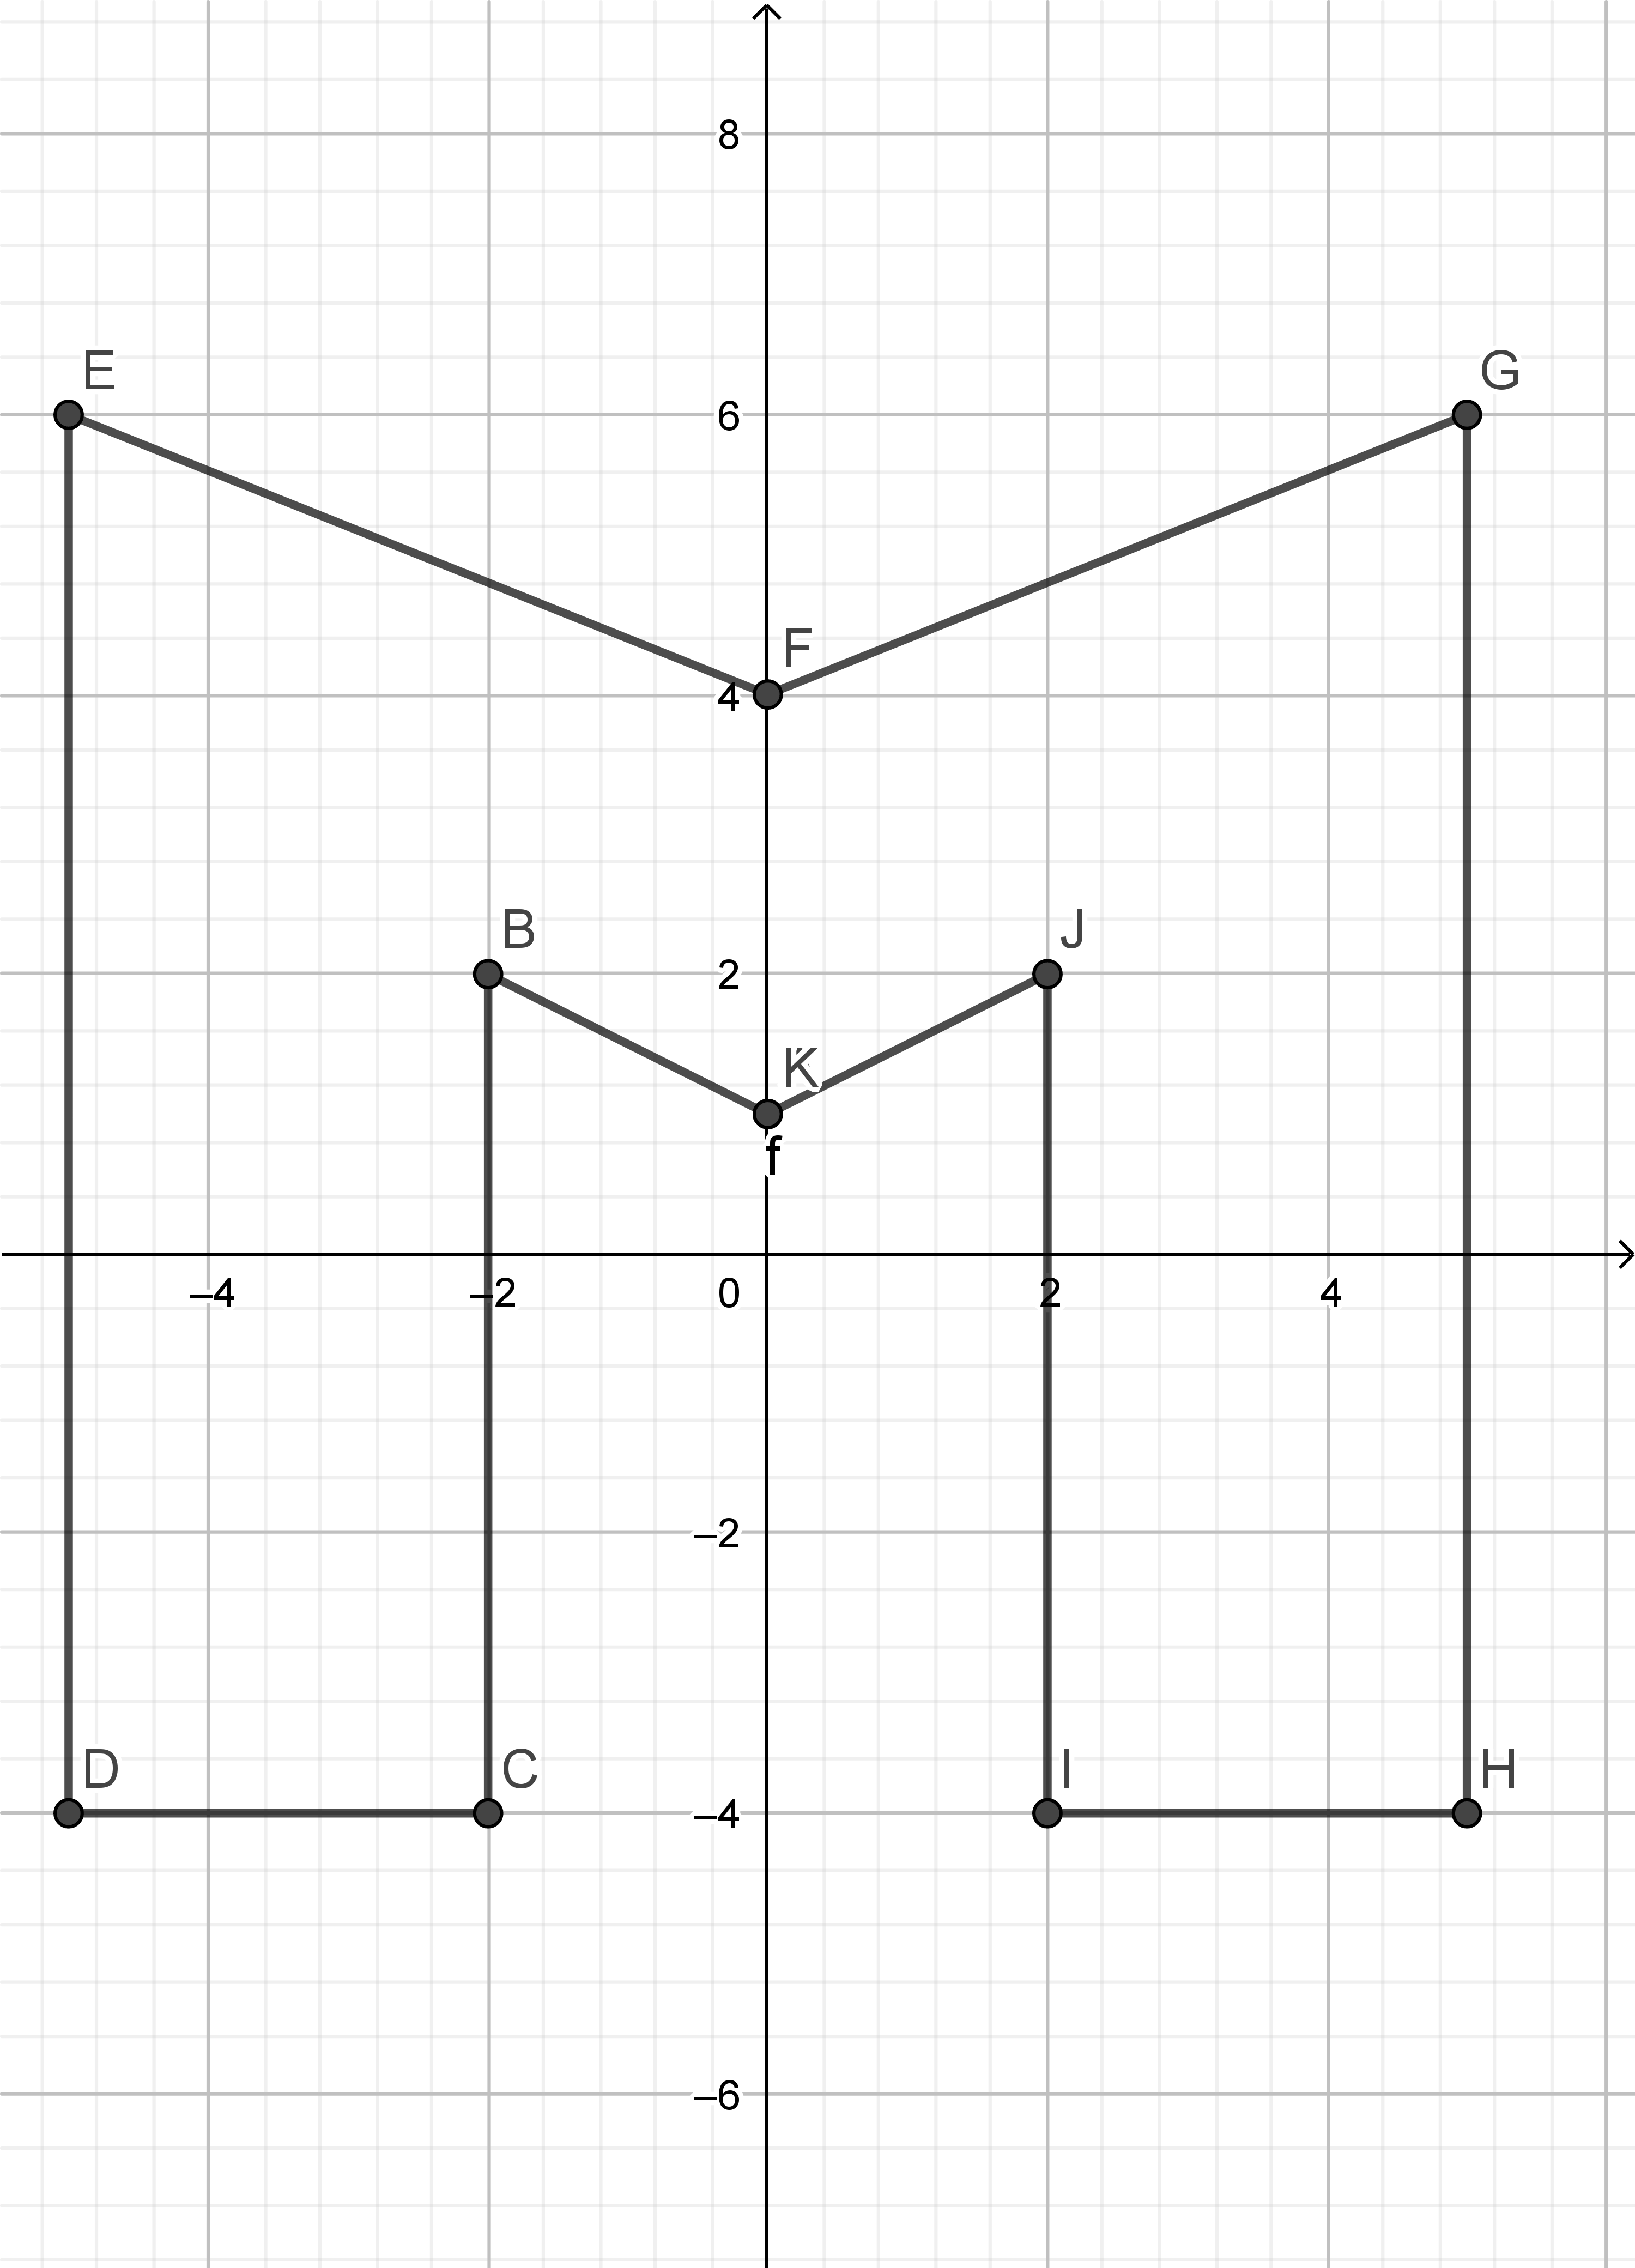
\includegraphics[width=60mm]{./images/ex3-letra-inicial.png}
                \caption{Letra inicial}
            \end{figure}
    
        \item
            Para a reflexão em torno do eixo y, usaremos
            \begin{equation}
                \begin{bmatrix} 
                -1 & 0 \\
                 0 & 1
                \end{bmatrix} 
                \cdot M = 
                \begin{bmatrix} 
                0 & 2 & 2 & 5 & 5 & 0 & -5  & -5 & -2 & -2 & 0 \\
                1 & 2 & -4&-4 & 6 & 4 & 6   & -4 & -4 &  2 & 1
                \end{bmatrix} 
            \end{equation}
        \item
            Para a o cisalhamento na horizontal, usaremos
            \begin{equation}
                \begin{bmatrix} 
                1 & 1/2 \\
                 0 & 1
                \end{bmatrix} 
                \cdot M = 
                \begin{bmatrix} 
                1/2 & -1 & -4 & -7 & -2 & 2 & 8  & 3 & 0 & 3 & 1/2 \\
                1 & 2 & -4&-4 & 6 & 4 & 6   & -4 & -4 &  2 & 1
                \end{bmatrix} 
            \end{equation}
            \begin{figure}[ht!]
                \centering
                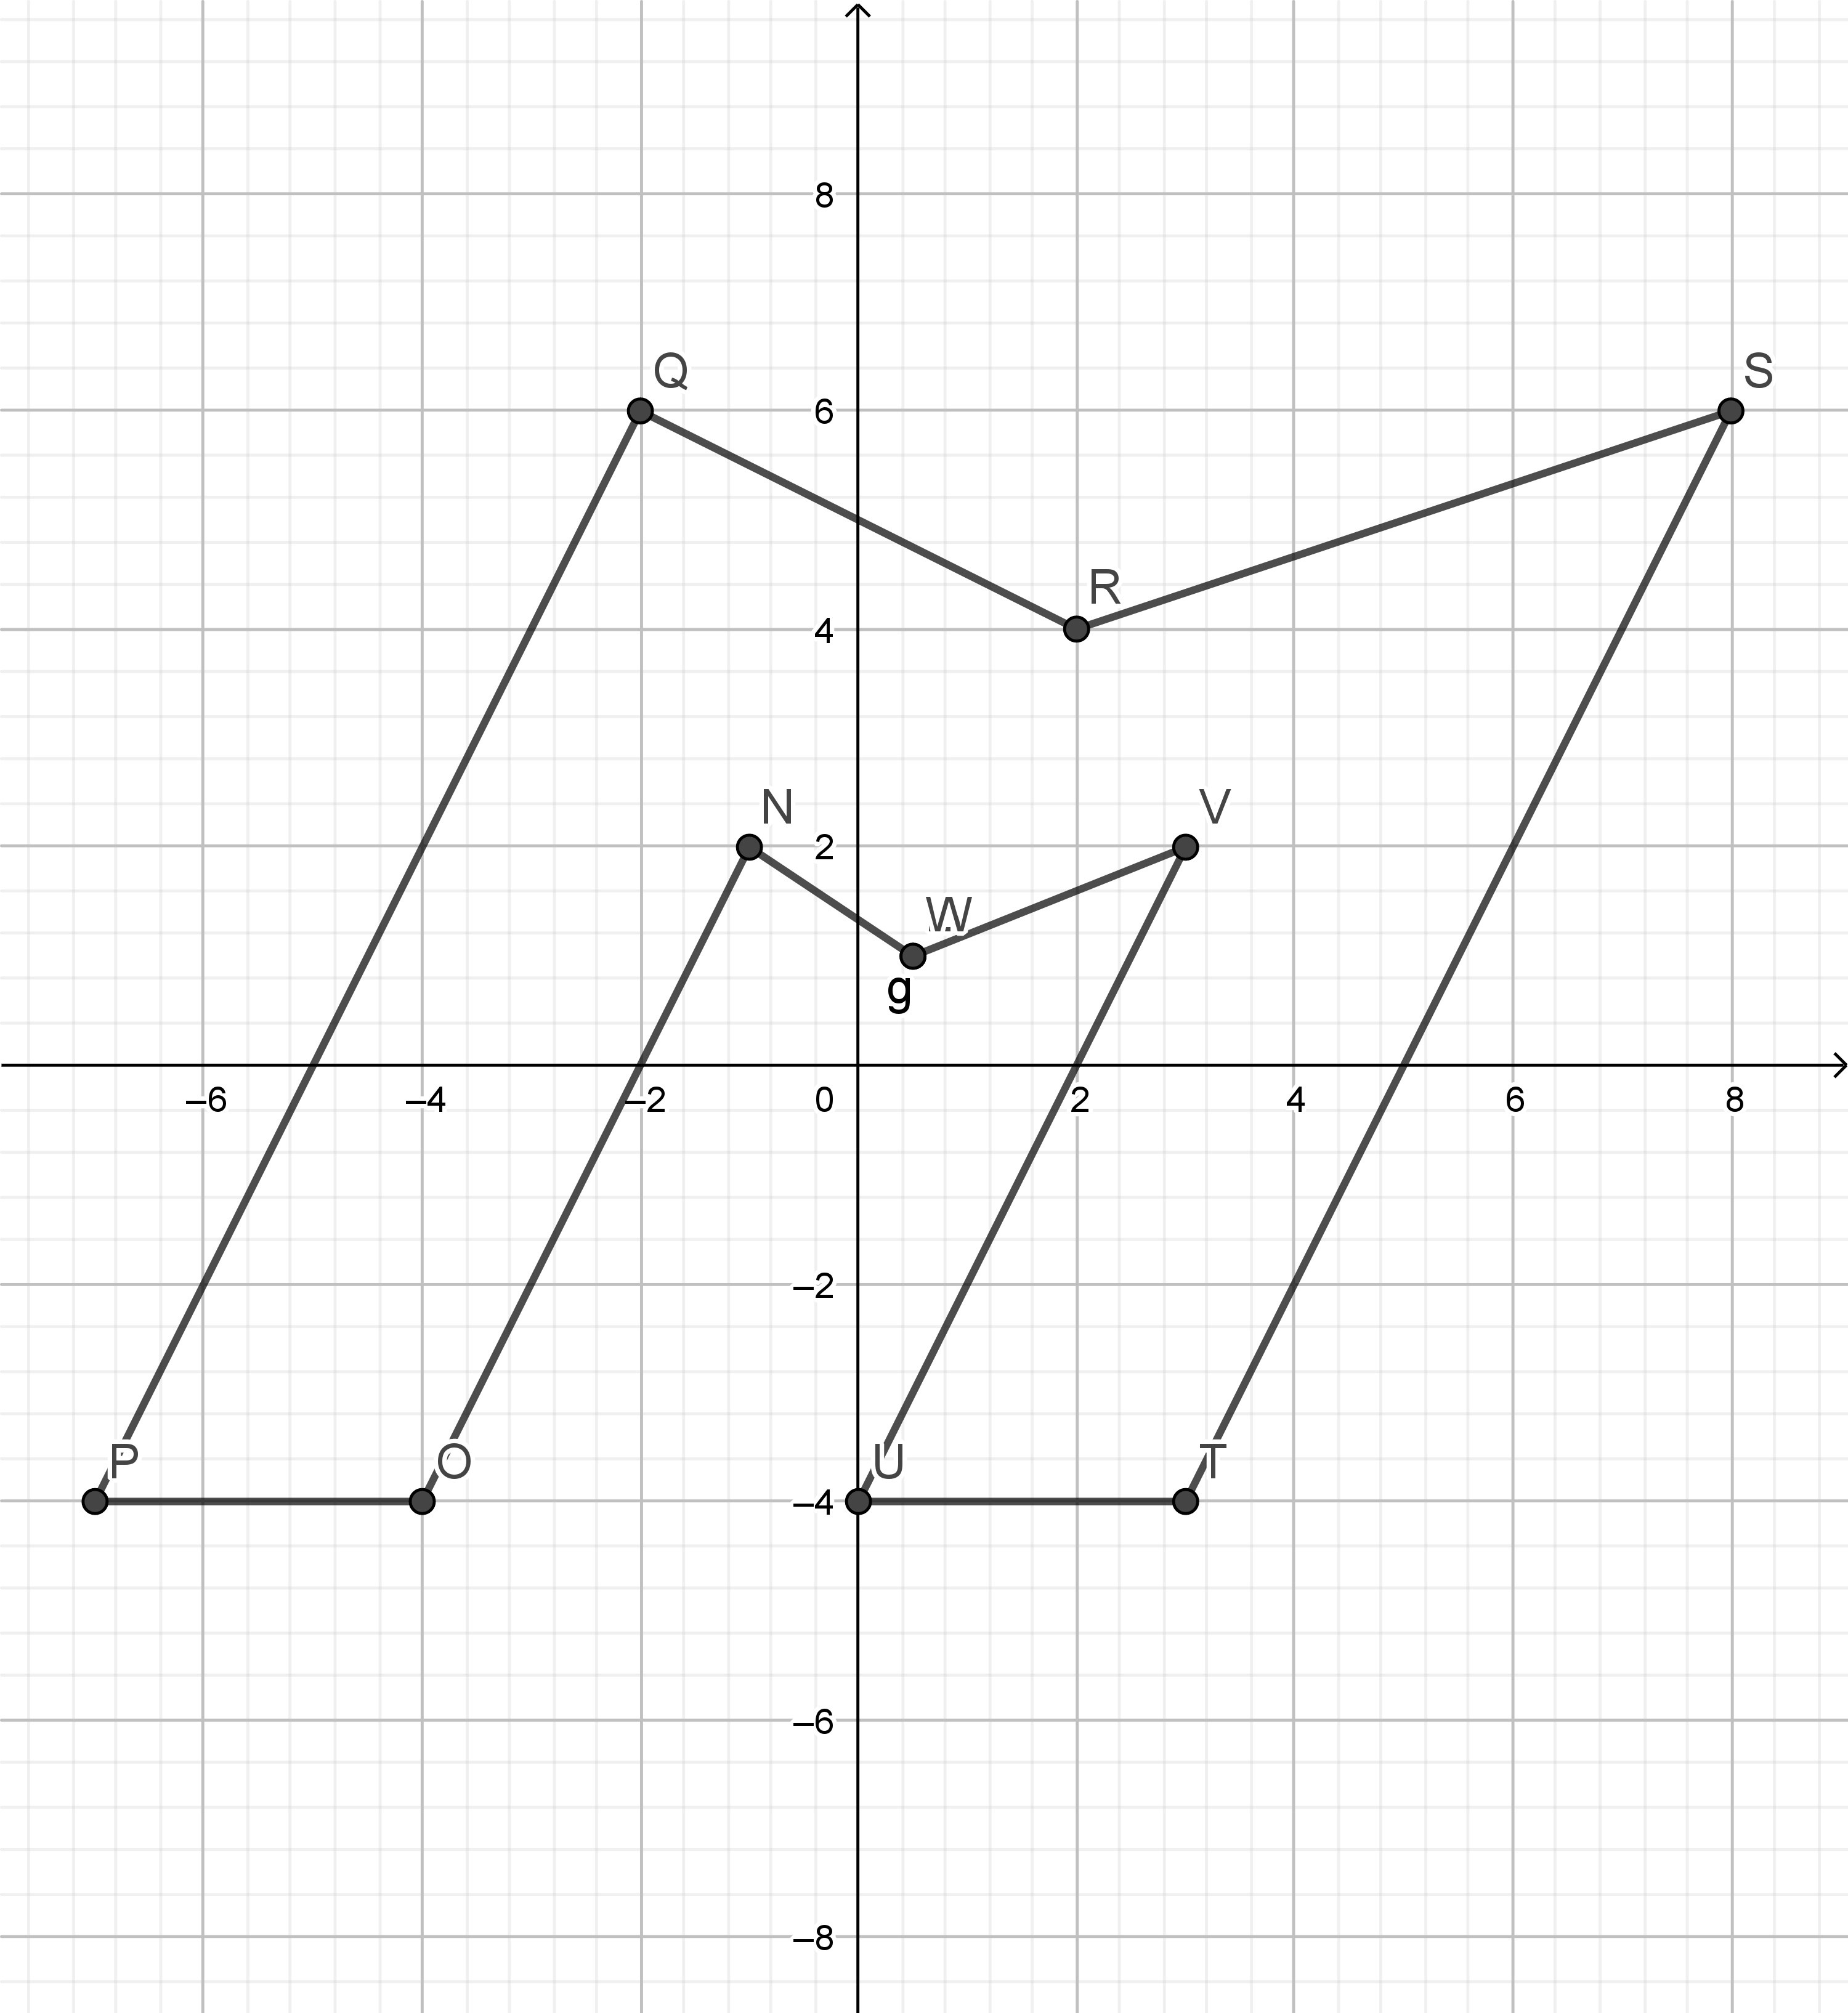
\includegraphics[width=60mm]{./images/ex3-cisalhamento.png}
                \caption{Cisalhamento na horizontal}
            \end{figure}

        \item 
            Para a reflexão em torno da reta $y = 3x$ primeiramente escolheremos uma base
            conveniente e verificaremos qual a imagem dos vetores da base. 
            Escolheremos a base $\beta = \{(1;3) ; (1;0)\}$, cujas imagens são: \\
            $(1;3) \rightarrow (1,3)$ \\
            $(1;0) \rightarrow (x_0; y_0)$ \\
            Sejam \\
            $f: \mathbb{R} \rightarrow \mathbb{R} ; f(x) = 3x$ e \\
            $g: \mathbb{R} \rightarrow \mathbb{R} ; g(x) = -3^{-1}x + b = \dfrac{-1}{3}x + b$ \\
            assim $f$ é a reta de reflexão e $g$ é uma função auxiliar. A ideia é que a reflexão
            de um ponto digamos, $P_1$, em torno de uma reta estará situado sobre a reta definida 
            pelos pontos $P_1$ e o pé da perpendicular ($P_2$) de $P_1$ em nossa reta, no caso $f$. \\
			\begin{tikzpicture}
                \draw[gray] (-2,2) grid[xstep=1, ystep=1]  (2,-2);
                \fill (1,0)  circle[radius=2pt];
                \node[below=3pt of {(1,0)}, outer sep=2pt,fill=white] {\tiny$ P_1(1,0)$};
                
                \fill (1/10,3/10)  circle[radius=2pt];
                \node[above right=2pt of {(1/10,3/10)}, outer sep=2pt,fill=white] {\tiny $P_2(\frac{1}{10},\frac{3}{10})$};

                \fill (-8/10,6/10)  circle[radius=2pt];
                \node[above=3pt of {(-8/10,6/10)}, outer sep=2pt,fill=white] {\tiny $P_3(\frac{-8}{10},\frac{6}{10})$};

                \draw[->][black] (-2,0) -- (2,0) node[right] {$x$};
                \draw[->][black] (0,-2) -- (0,2) node[above] {$y$};

                \draw[scale=1,domain=-7/10:7/10,smooth,variable=\x,blue] plot ({\x},{3 *\x});
                \node[below=2pt of {(0.7,2)}, outer sep=2pt, color=blue] {\tiny $f$};

                \draw[scale=1,domain=-2:2,smooth,variable=\x,red] plot ({\x},{-1/3 *\x + 1/3});
                \node[below=2pt of {(-0.7,0.5)}, outer sep=2pt, color=red] {\tiny $g$};

			\end{tikzpicture} \\
            Ainda, $P_3$ é tal que $P_2$ seja o ponto médio de $P_1$ e $P_3$, 
            logo $P_3 = (\frac{1}{10} - \abs{1-\frac{1}{10}} ; y) = \Big( \frac{-8}{10} ; g(\frac{-8}{10}) \Big) = \Big( \frac{-8}{10} ; \frac{6}{10} \Big)$.
            O coeficiente angular de $g$ obtemos facilmente lembrando que no caso de funções que descrevem retas, 
            elas são perpendiculares se, e somente se o produto dos coeficientes lineares for igual a $-1$. O coeficiente linear obtemos
            usando o coeficiente angular com o ponto $P_1$. Com isso obtemos $g(x) = \frac{-1}{3}x+\frac{1}{3}$. $P_2$ 
            é a intersecção das duas retas, logo:
            \begin{equation}
                f(x) = g(x) \iff
                3x = \frac{-1}{3} x + \frac{1}{3} \iff
                x = \frac{1}{10}
            \end{equation}
            Ainda, $P_2 = (\frac{1}{10}, f(\frac{1}{10}) ) = (\frac{1}{10};\frac{3}{10})$
            Agora encontremos os coeficientes da matriz tranformação:
            \begin{equation}
                \begin{bmatrix}
                a & b \\
                c & d \\
                \end{bmatrix}
                \cdot
                \begin{bmatrix}
                1 \\
                3 \\
                \end{bmatrix}
                =
                \begin{bmatrix}
                1 \\
                3 \\
                \end{bmatrix}
            \end{equation}
            \begin{equation}
                \begin{bmatrix}
                a & b \\
                c & d \\
                \end{bmatrix}
                \cdot
                \begin{bmatrix}
                1 \\
                0 \\
                \end{bmatrix}
                =
                \begin{bmatrix}
                \frac{-8}{10} \\
                \frac{6}{10} \\
                \end{bmatrix}
            \end{equation}
            Chegamos ao sistema:

            \systeme*{{a + 3b = 1}, {c + 3d = 3}, {a = \frac{-8}{10}}, {c = \frac{6}{10}}} \\
            Resolvendo chegamos na matriz:
            \begin{equation}
            \begin{bmatrix}
                \frac{-8}{10} & \frac{3}{5} \\
                \frac{6}{10} & \frac{4}{5} \\
            \end{bmatrix}
                \iff T(x;y) = \Big( \frac{-8}{10}x + \frac{3}{5}y ; \frac{6}{10}x + \frac{4}{5}y \Big)
            \end{equation}
            \begin{figure}[ht!]
                \centering
                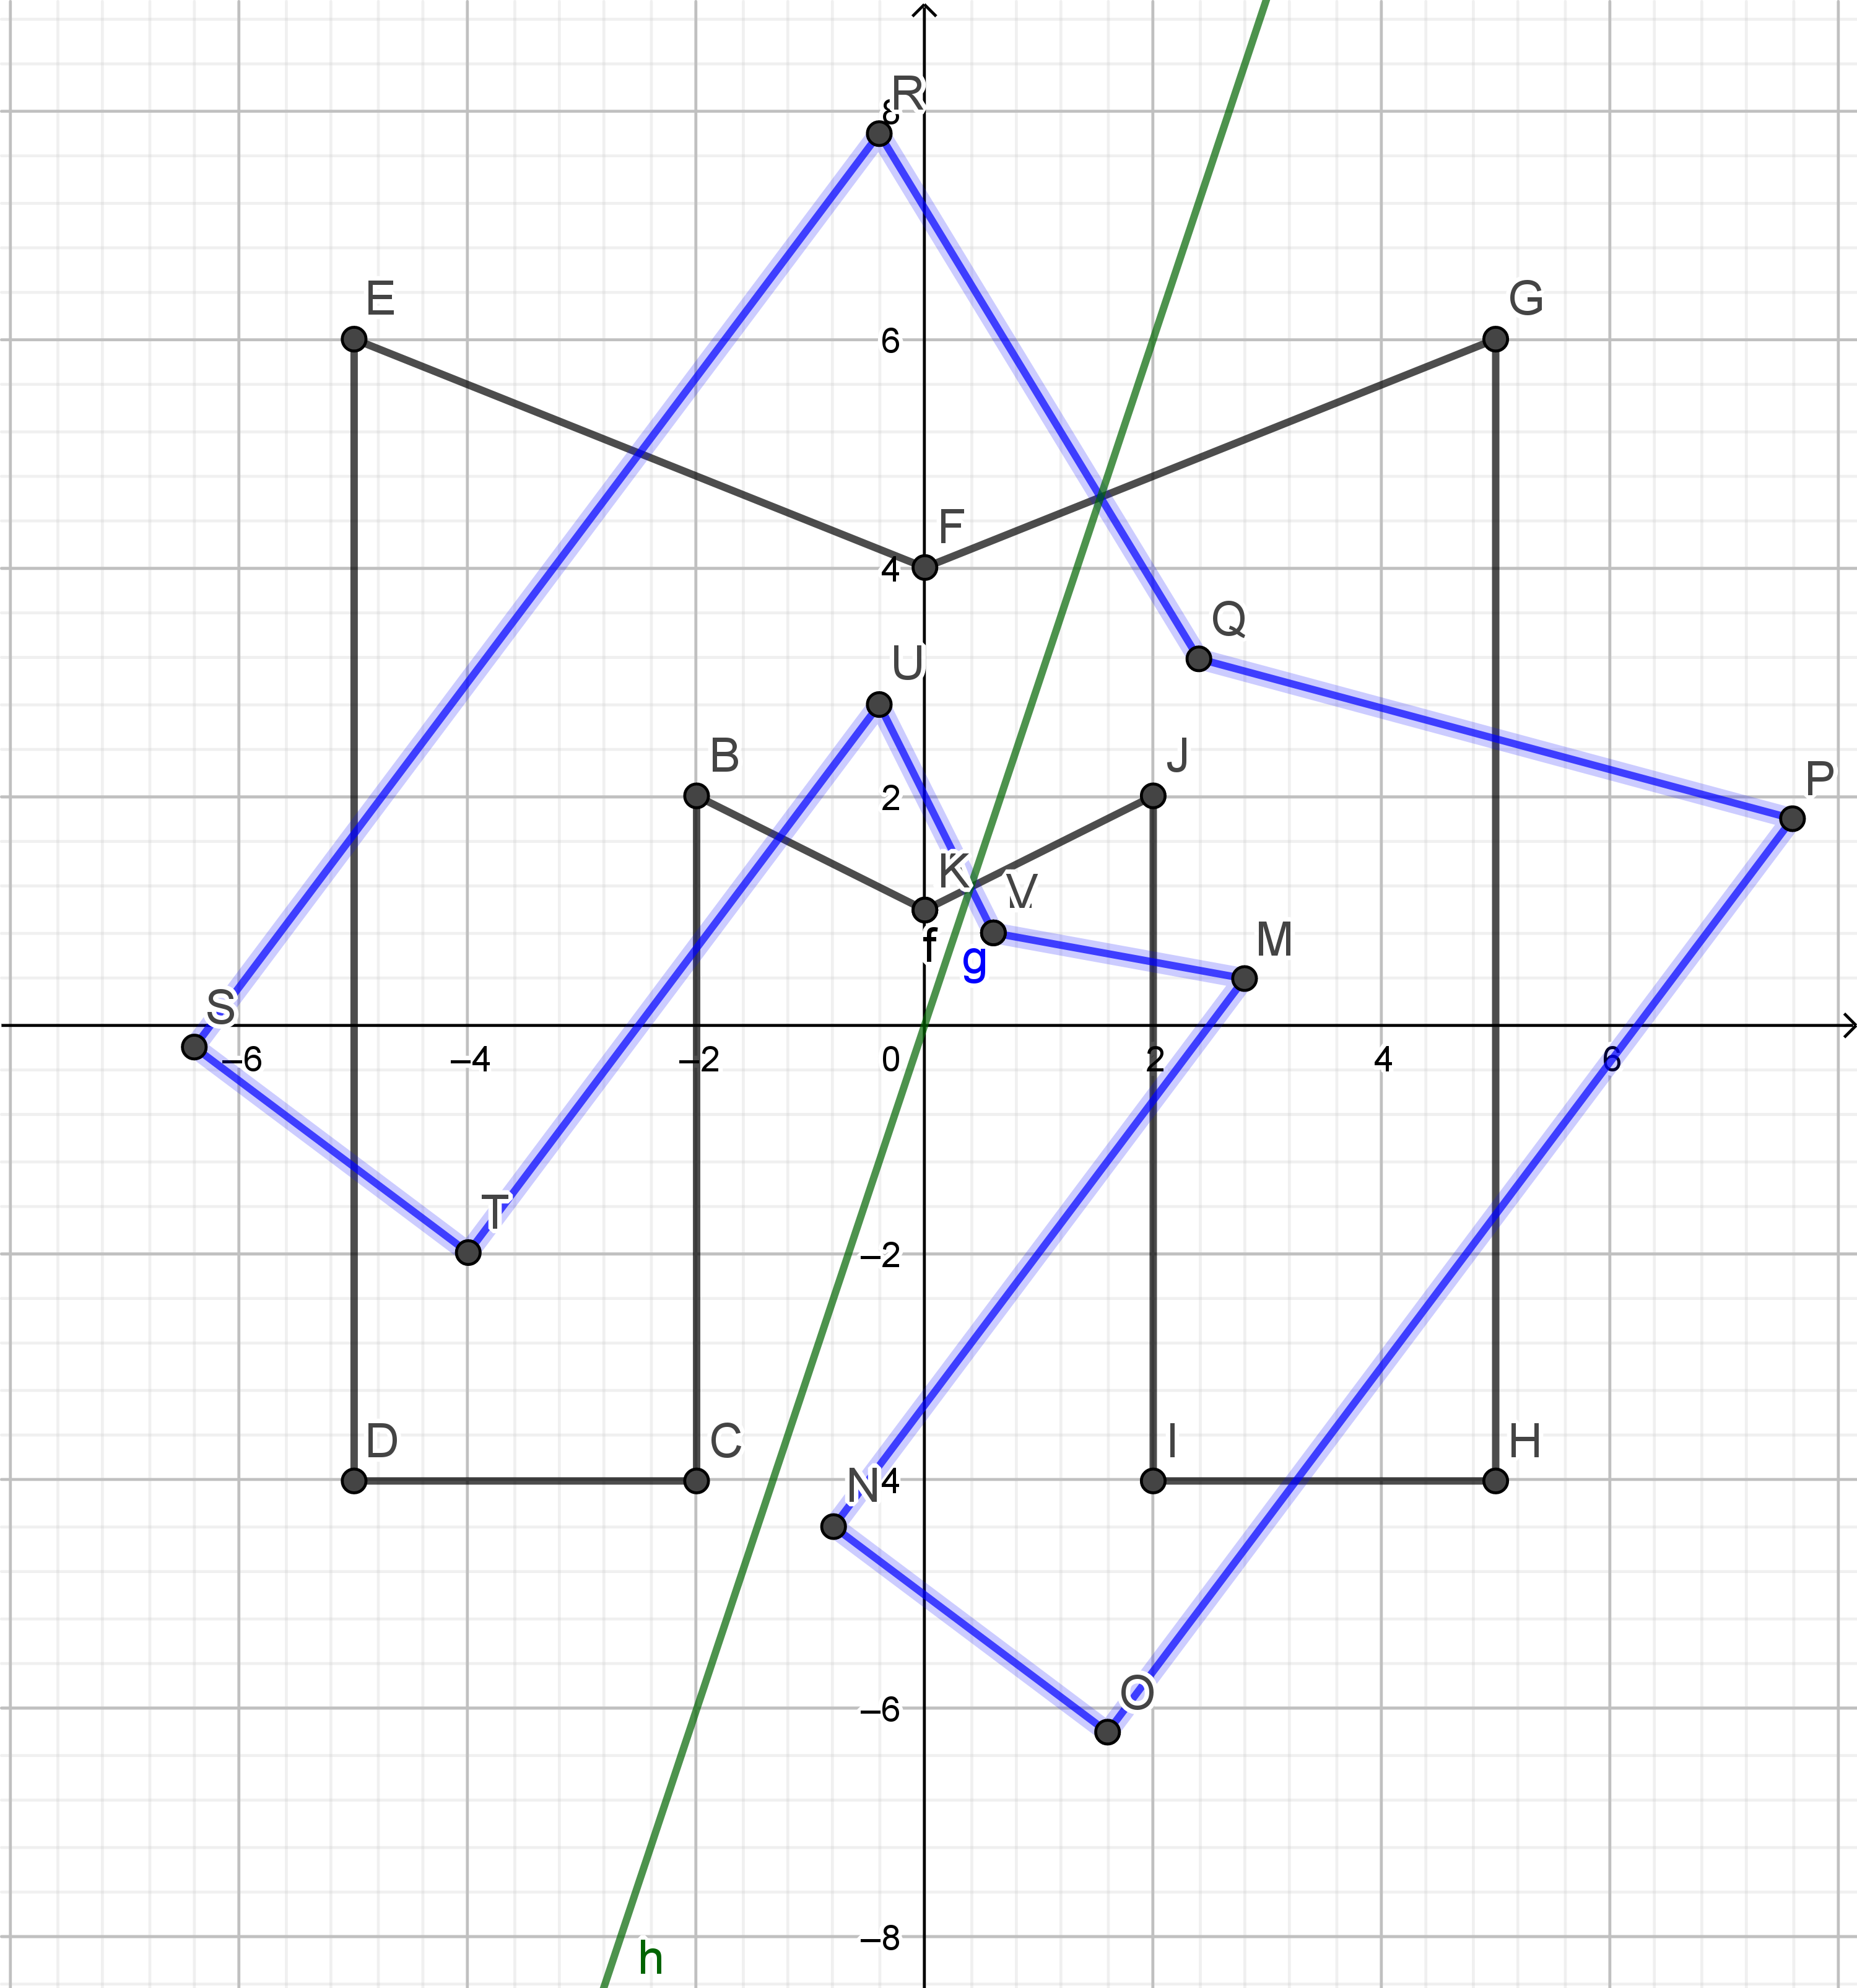
\includegraphics[width=80mm]{./images/ex3-c-c-reflexao-na-reta.png}
                \caption{Reflexão em torno de $y=3x$}
            \end{figure}
        \end{enumerate}

    \item
        \begin{enumerate}
            \item
                Considerando os pontos $B, E$ temos:\\
                $T(E) = T(0;2) = (2;6) \\
                 T(B) = T(1;-1) = (2; -2)$

                \begin{equation}
                    \begin{bmatrix}
                    a & b \\
                    c & d \\
                    \end{bmatrix}
                    \cdot
                    \begin{bmatrix}
                    0 \\
                    2 \\
                    \end{bmatrix}
                    =
                    \begin{bmatrix}
                    2 \\
                    6
                    \end{bmatrix}
                \end{equation}
                \begin{equation}
                    \begin{bmatrix}
                    a & b \\
                    c & d \\
                    \end{bmatrix}
                    \cdot
                    \begin{bmatrix}
                    1 \\
                    -1 \\
                    \end{bmatrix}
                    =
                    \begin{bmatrix}
                    2 \\
                    -2
                    \end{bmatrix}
                \end{equation}
                Chegamos ao sistema:
                \systeme*{{2b = 1}, {2d = 6}, {a = 3}, {c = 1}} \\
                \begin{equation}
                    \begin{bmatrix}
                        a&b \\
                        c&d \\
                    \end{bmatrix}
                    =
                    \begin{bmatrix}
                        3&1 \\
                        1&3 \\
                    \end{bmatrix}
                    \iff T(x;y) = (3x+y ; x+3y)
                \end{equation}
            \item
                \begin{equation}
                    \begin{bmatrix}
                        3 - \lambda & 1 \\
                        1 & 3 - \lambda \\
                    \end{bmatrix}
                    = Z \leadsto \\
                    det Z = (3 - \lambda)^2 -1 = (\lambda -2)(\lambda -4)
                \end{equation}
                Logo os autovalores são $\{2, 4\}$, pois zeram o polinômio característico.
                \begin{equation}
                    \begin{bmatrix}
                        3 - 2 & 1 \\
                        1 & 3 - 2 \\
                    \end{bmatrix}
                    =
                    \begin{bmatrix}
                        1 & 1 \\
                        1 & 1 \\
                    \end{bmatrix}
                    \leadsto 
                    \begin{bmatrix}
                        1 & 1 \\
                        1 & 1 \\
                    \end{bmatrix}
                    \begin{bmatrix}
                        x \\
                        y
                    \end{bmatrix}
                    \begin{bmatrix}
                        0 \\
                        0
                    \end{bmatrix}
                    \implies x + y = 0 \leadsto \beta_{\lambda=2} = \{(1;-1)\}
                \end{equation}

                \begin{equation}
                    \begin{bmatrix}
                        3 - 4 & 1 \\
                        1 & 3 - 4 \\
                    \end{bmatrix}
                    =
                    \begin{bmatrix}
                        -1 & 1 \\
                        1 & -1 \\
                    \end{bmatrix}
                    \leadsto 
                    \begin{bmatrix}
                        -1 & 1 \\
                        1 & -1 \\
                    \end{bmatrix}
                    \begin{bmatrix}
                        x \\
                        y
                    \end{bmatrix}
                    \begin{bmatrix}
                        0 \\
                        0
                    \end{bmatrix}
                    \implies x - y = 0 \leadsto \beta_{\lambda=4} = \{(1;1)\}
                \end{equation}
                Assim, os autovetores (que $T(u)$ ficam na mesma direção que $u$) são múltiplos de $(1;-1)$ ou múltiplos de $(1;1)$,
                e ficam ampliados ou reduzidos pelo módulo do autovalor correspondente (autovalor que nos permitiu encontrar a base).
                E o sentido varia de acordo com o sinal do autovalor.
            \item
            \begin{figure}[ht!]
                \centering
                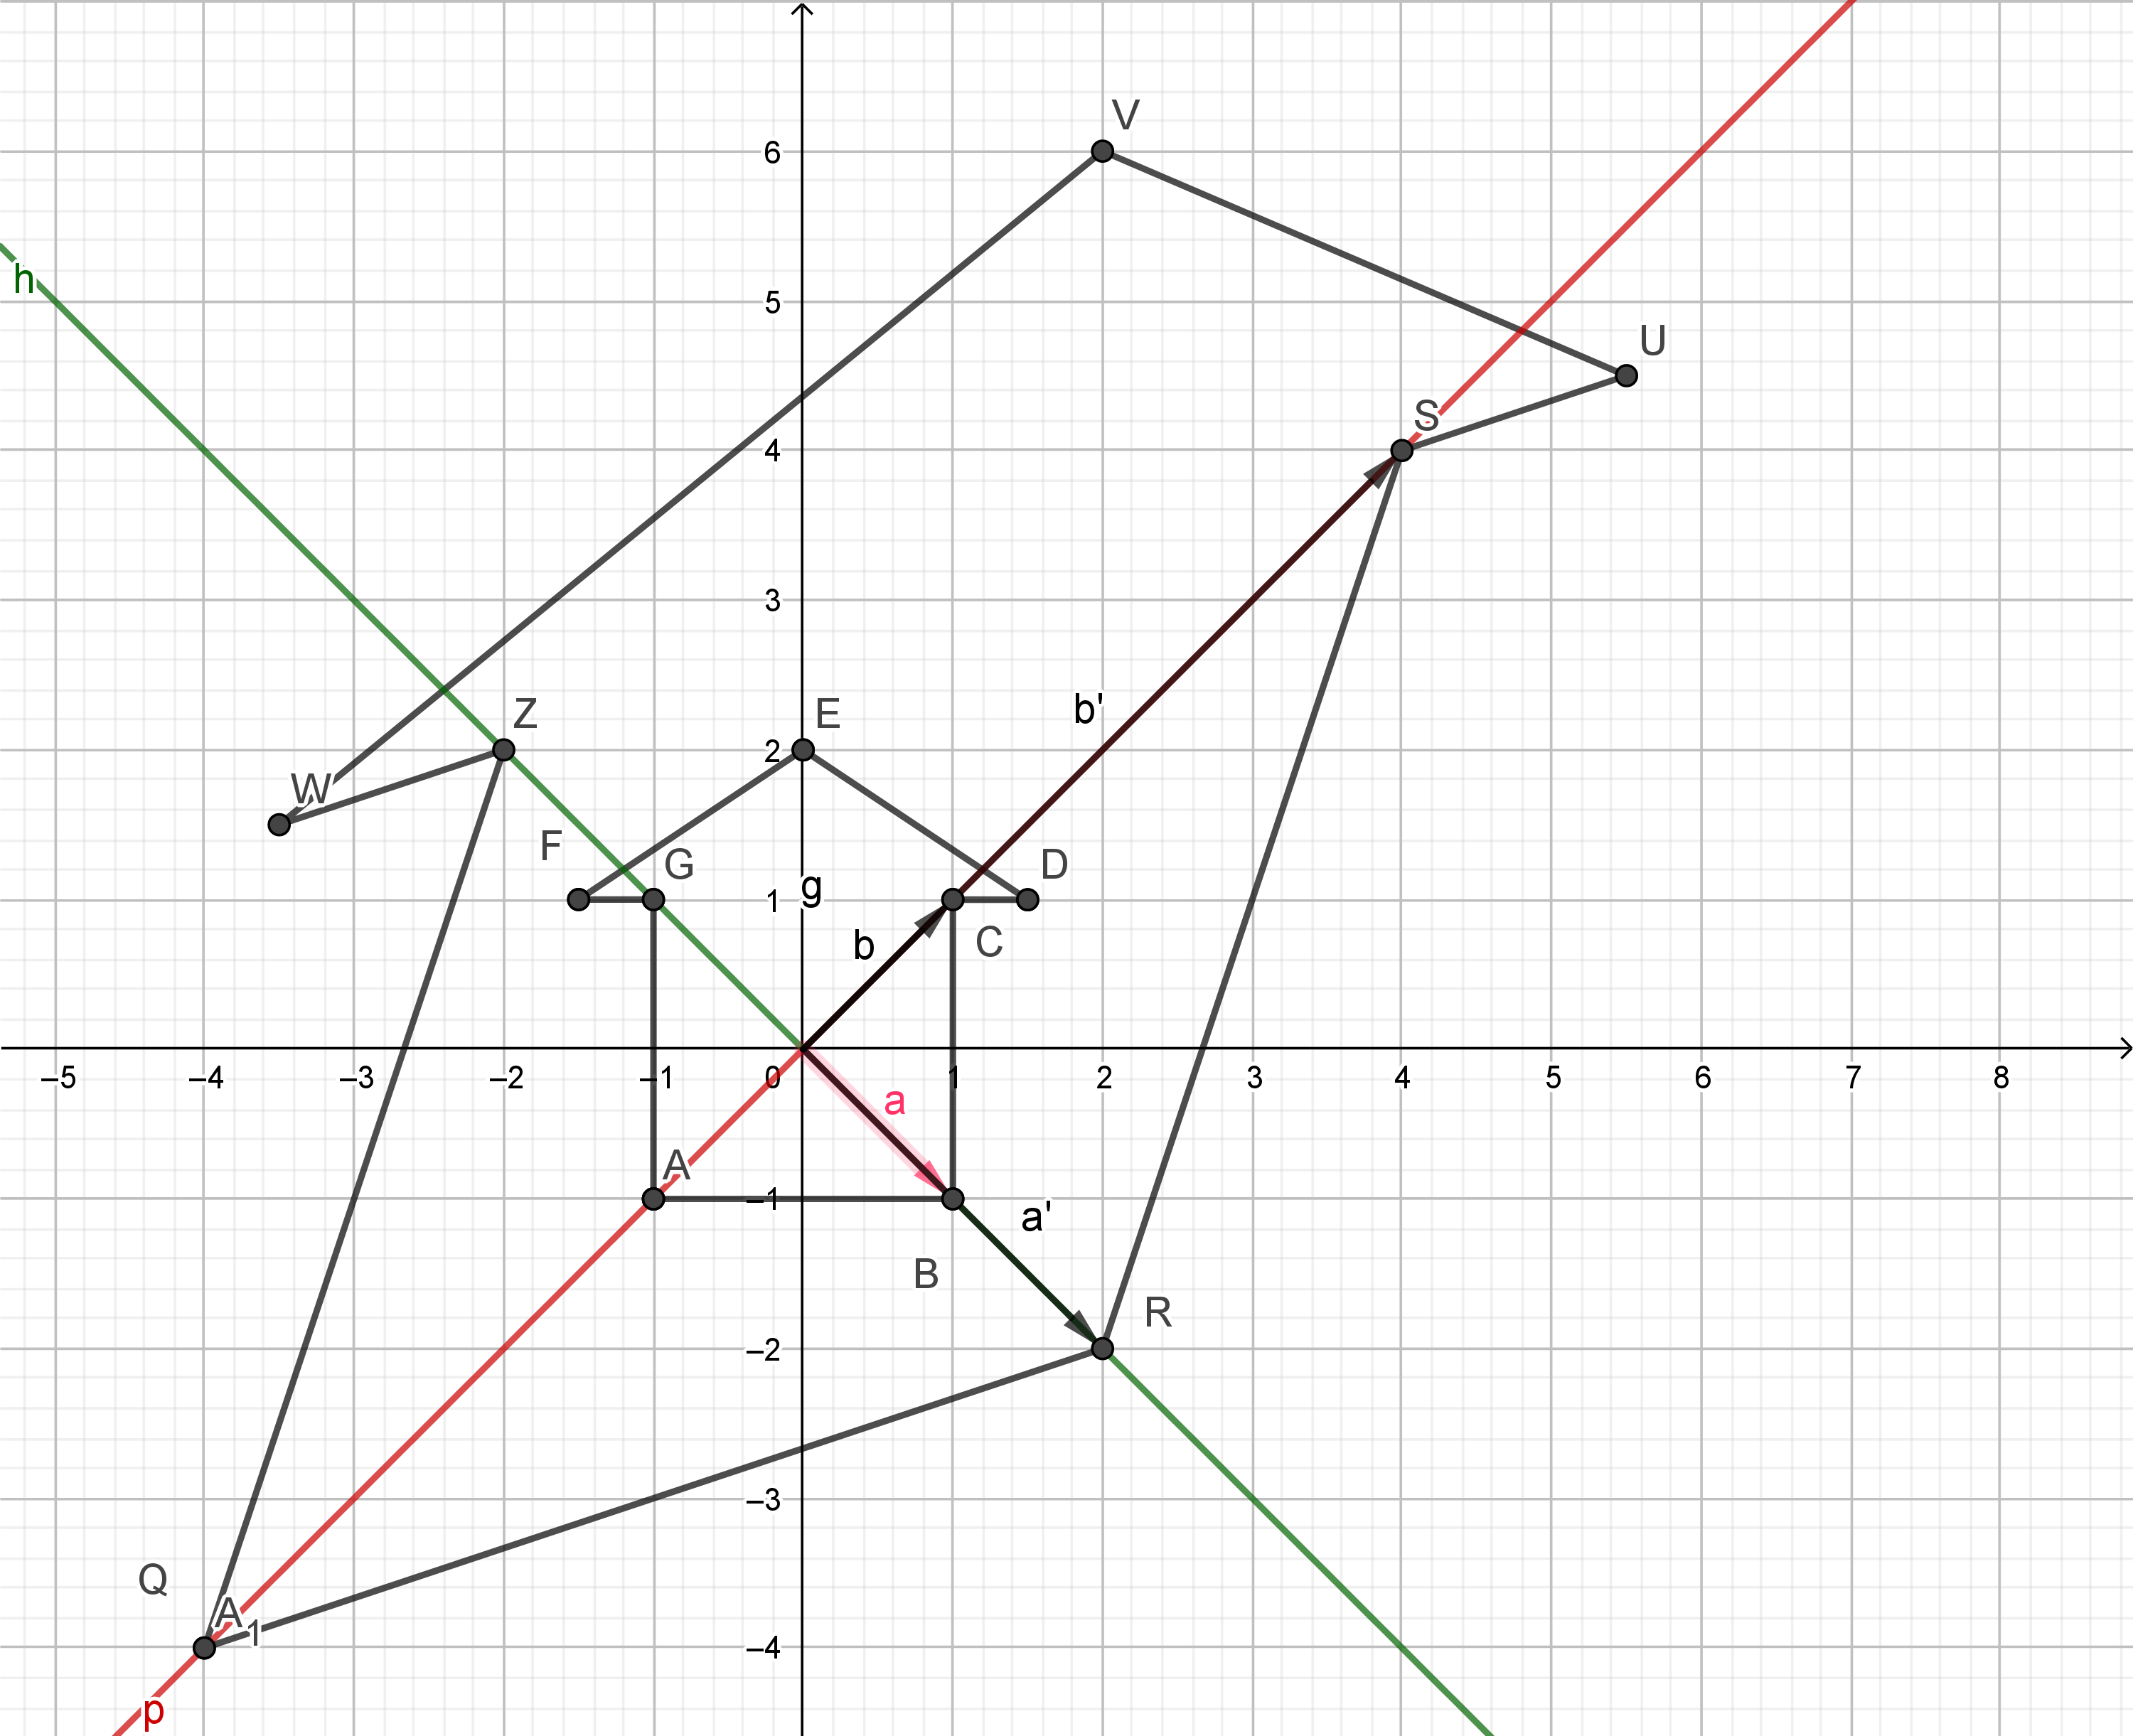
\includegraphics[width=100mm]{./images/ex4-final.png}
                \caption{Representação da transformação e autovetores}
            \end{figure}
            Os vetores nas retas $p, h$ são transformados em vetores que tem a mesma direção dos vetores iniciais. Por exemplo,
            $T(a) = a'$ e $T(b) = b'$. Peguei vetores de cada base mas poderia ter pego qualquer multiplo que estivessem sobre $p$ ou $h$.

        \end{enumerate}
    %%%%%%%%%% Exercício 1 - Início
    %\item
        %Vamos encontrar um parabolóide que satisfaça a condição exigida.
        %Sabendo que um parabolóide qualquer pode ser expresso por:
        %$$ p: c_1 \cdot \left( x - a \right)^2 + c_2 \cdot \left( y - b\right)^2 + d = z$$
        %Onde $c_1, c_2, a, b \in \mathbb{R} \land c_1 \cdot c_2 > 0$ \\
        %Com a equação do plano dada: $ \pi: 13x - 8y - z = 24 \iff 13x -8y -24 = z$ podemos obter o vetor normal, 
        %$\overrightarrow{n} = (-13, +8, +1)$. 
%
        %\systeme*{{-13 = -\dfrac{\partial f}{\partial x} (1,2)},,{+8 = -\dfrac{\partial f}{\partial y} (1,2)}}
        %$$ -13 = -\dfrac{\partial f}{\partial x} (1,2) \implies 2c_1 - 2c_1a = +13$$
        %$$ +8 = -\dfrac{\partial f}{\partial y} (1,2) \implies 4c_2 - 2c_2b = -8$$
        %Substituindo com qualquer par de números reais tais que $c_1 \cdot c_2 > 0$, escolheremos $c_1 = 3$ e $c_2 = 7$ então:
        %$$ 2 \cdot 3 - 2 \cdot 3 \cdot a = 13 \implies a = \dfrac{-7}{6}$$
        %$$ 4 \cdot 7 - 2 \cdot 7 \cdot b = -8 \implies b = \dfrac{18}{7}$$
        %E assim temos a equação:
        %$$ 3 \left( x + \dfrac{7}{6} \right)^2 + 7 \left( y - \dfrac{18}{7} \right)^2 + d = z $$
        %E para encontrar $d$ basta substituir as variáveis da equação no ponto que desejamos que pertença a esse parabolóide.
        %Então segue:
        %$$ 3 \left( 1 + \dfrac{7}{6} \right)^2 + 7 \left( 2 - \dfrac{18}{7} \right)^2 + d = -27 $$
        %$$ \dfrac{169}{12} +\dfrac{16}{7} + d = -27 \implies d = \dfrac{-3643}{84}$$
        %Temos agora a equação que procurávamos, que é dada por:
        %$$ 3 \left( x + \dfrac{7}{6} \right)^2 + 7 \left( y - \dfrac{18}{7} \right)^2 -\dfrac{3643}{84} = z $$
        %A figura está representada abaixo na figura \ref{exercicio1}:
        %\begin{figure}[ht!]
            %\centering
            %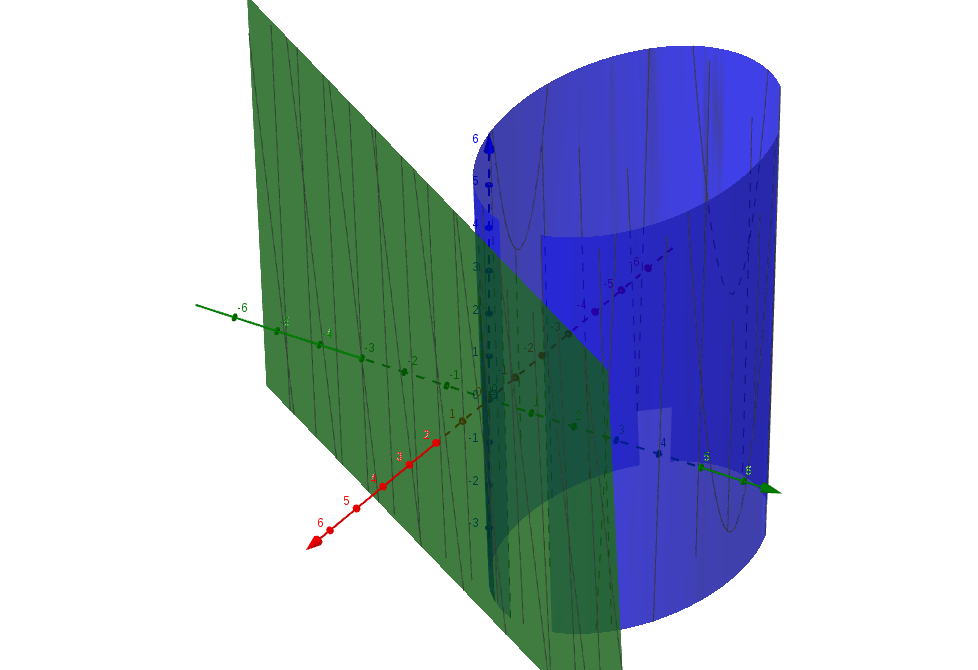
\includegraphics[width=90mm]{./images/exercicio1.png}
            %\caption{Plano e parabolóide\label{exercicio1}}
        %\end{figure}
%\newpage
    %%%%%%%%%%% Exercício 1 - Fim
%
    %%%%%%%%% Exercício 2 - Início
    %\item
        %Vamos chamar o sólido por corneta. 
        %Ela é representada na figura \ref{solido}:
%
        %\begin{figure}[ht!]
            %\centering
            %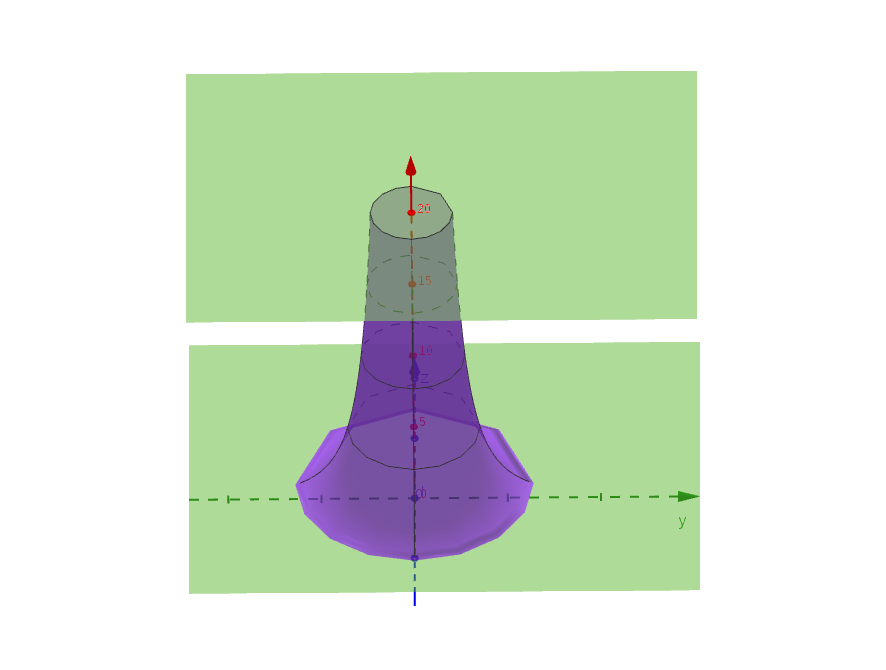
\includegraphics[width=90mm]{./images/3d-solido.png}
            %\caption{Corneta \label{solido}}
        %\end{figure}
        %
        %Construiremos o sólido tem torno do eixo $x$.
        %A figura é delimitada por dois planos, a saber $x = 1$ e $x = 20$. \\
        %Chamando \\
        %$
        %d_1 = 1 , \\
        %d_2 = 5 + d_1 = 6, \\
        %d_3 = 5 + d_2 = 11, \\
        %d_4 = 5 + d_3 = 16, \\
        %d_5 = 4 + d_3 = 20$ \\
        %Seja $I_n = \{x \in \mathbb{N}; x \leq n\}$ \\
        %Tomando os planos $p_n: x = d_n, n \in I_5$ temos eles 
        %representados abaixo na figura \ref{3d-planos-dn}:
%
        %\begin{figure}[ht!]
            %\centering
            %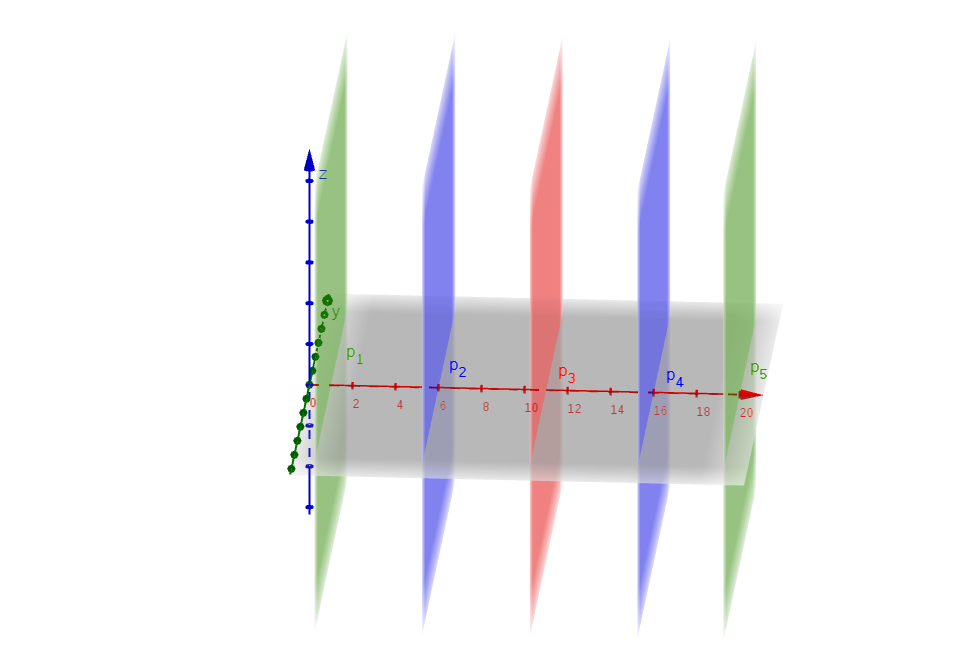
\includegraphics[width=90mm]{./images/3d-planos-dn.png}
            %\caption{Planos definidos por $d_n$ \label{3d-planos-dn}}
        %\end{figure}
    %
        %Sejam então os raios aproximados das mensurações (os denominadores representam o diâmetro): \\
        %$$ r_1 = \dfrac{13}{2} \approx 6.5,$$ 
        %$$ r_2 = \displaystyle \dfrac{7}{2} \approx 3.5, $$
        %$$r_3 = \dfrac{6}{2} \approx 3,$$
        %$$r_4 = \dfrac{4.7}{2} \approx 2.35,$$
        %$$r_5 = \dfrac{4.5}{2} \approx 2.25$$
%
        %Essas circunferências foram obtidas da seguinte forma:
        %$$c_n: x = d_n  \land r_n^2 = y^2 + z^2 \implies x = d_n = \dfrac{d_n}{r_n^2} \cdot \left( y^2 + z^2 \right)$$
        %Então fazemos a interseção da circunferência com o plano $xy$, que nos 
        %fornecerá os pontos $A_n, B_n, ..., E_n$ como mostra a figura \ref{3d-intersecao-circ-xy}:
%
        %\begin{figure}[ht!]
            %\centering
            %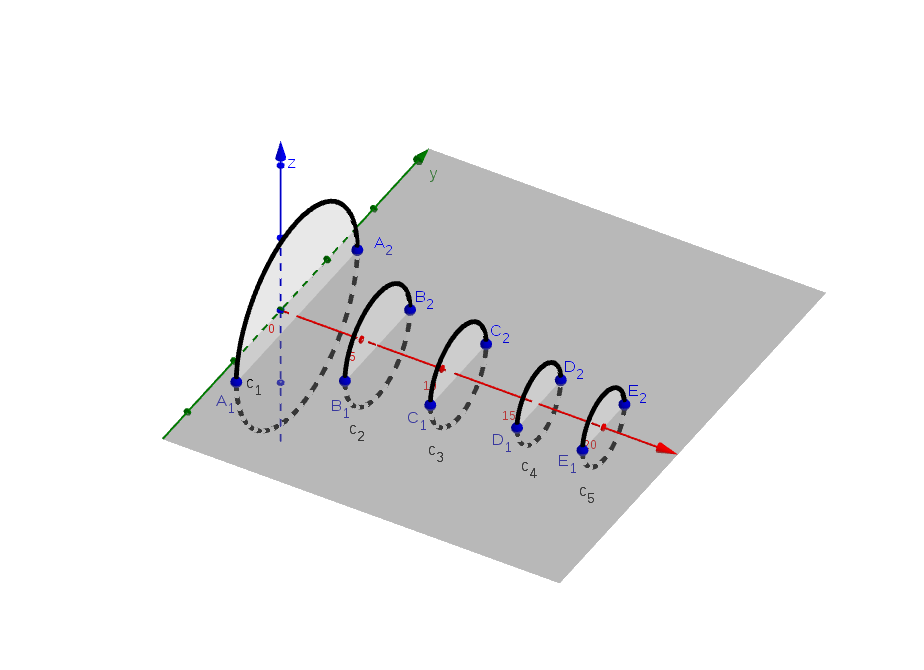
\includegraphics[width=90mm]{./images/3d-intersecao-circ-xy.png}
            %\caption{Interseção das circunferências com o plano $xy$ \label{3d-intersecao-circ-xy}}
        %\end{figure}
%
        %Consequentemente, no plano $xy$ os pontos são mostrados na figura \ref{figu}:
%
        %\begin{figure}[ht!]
            %\centering
            %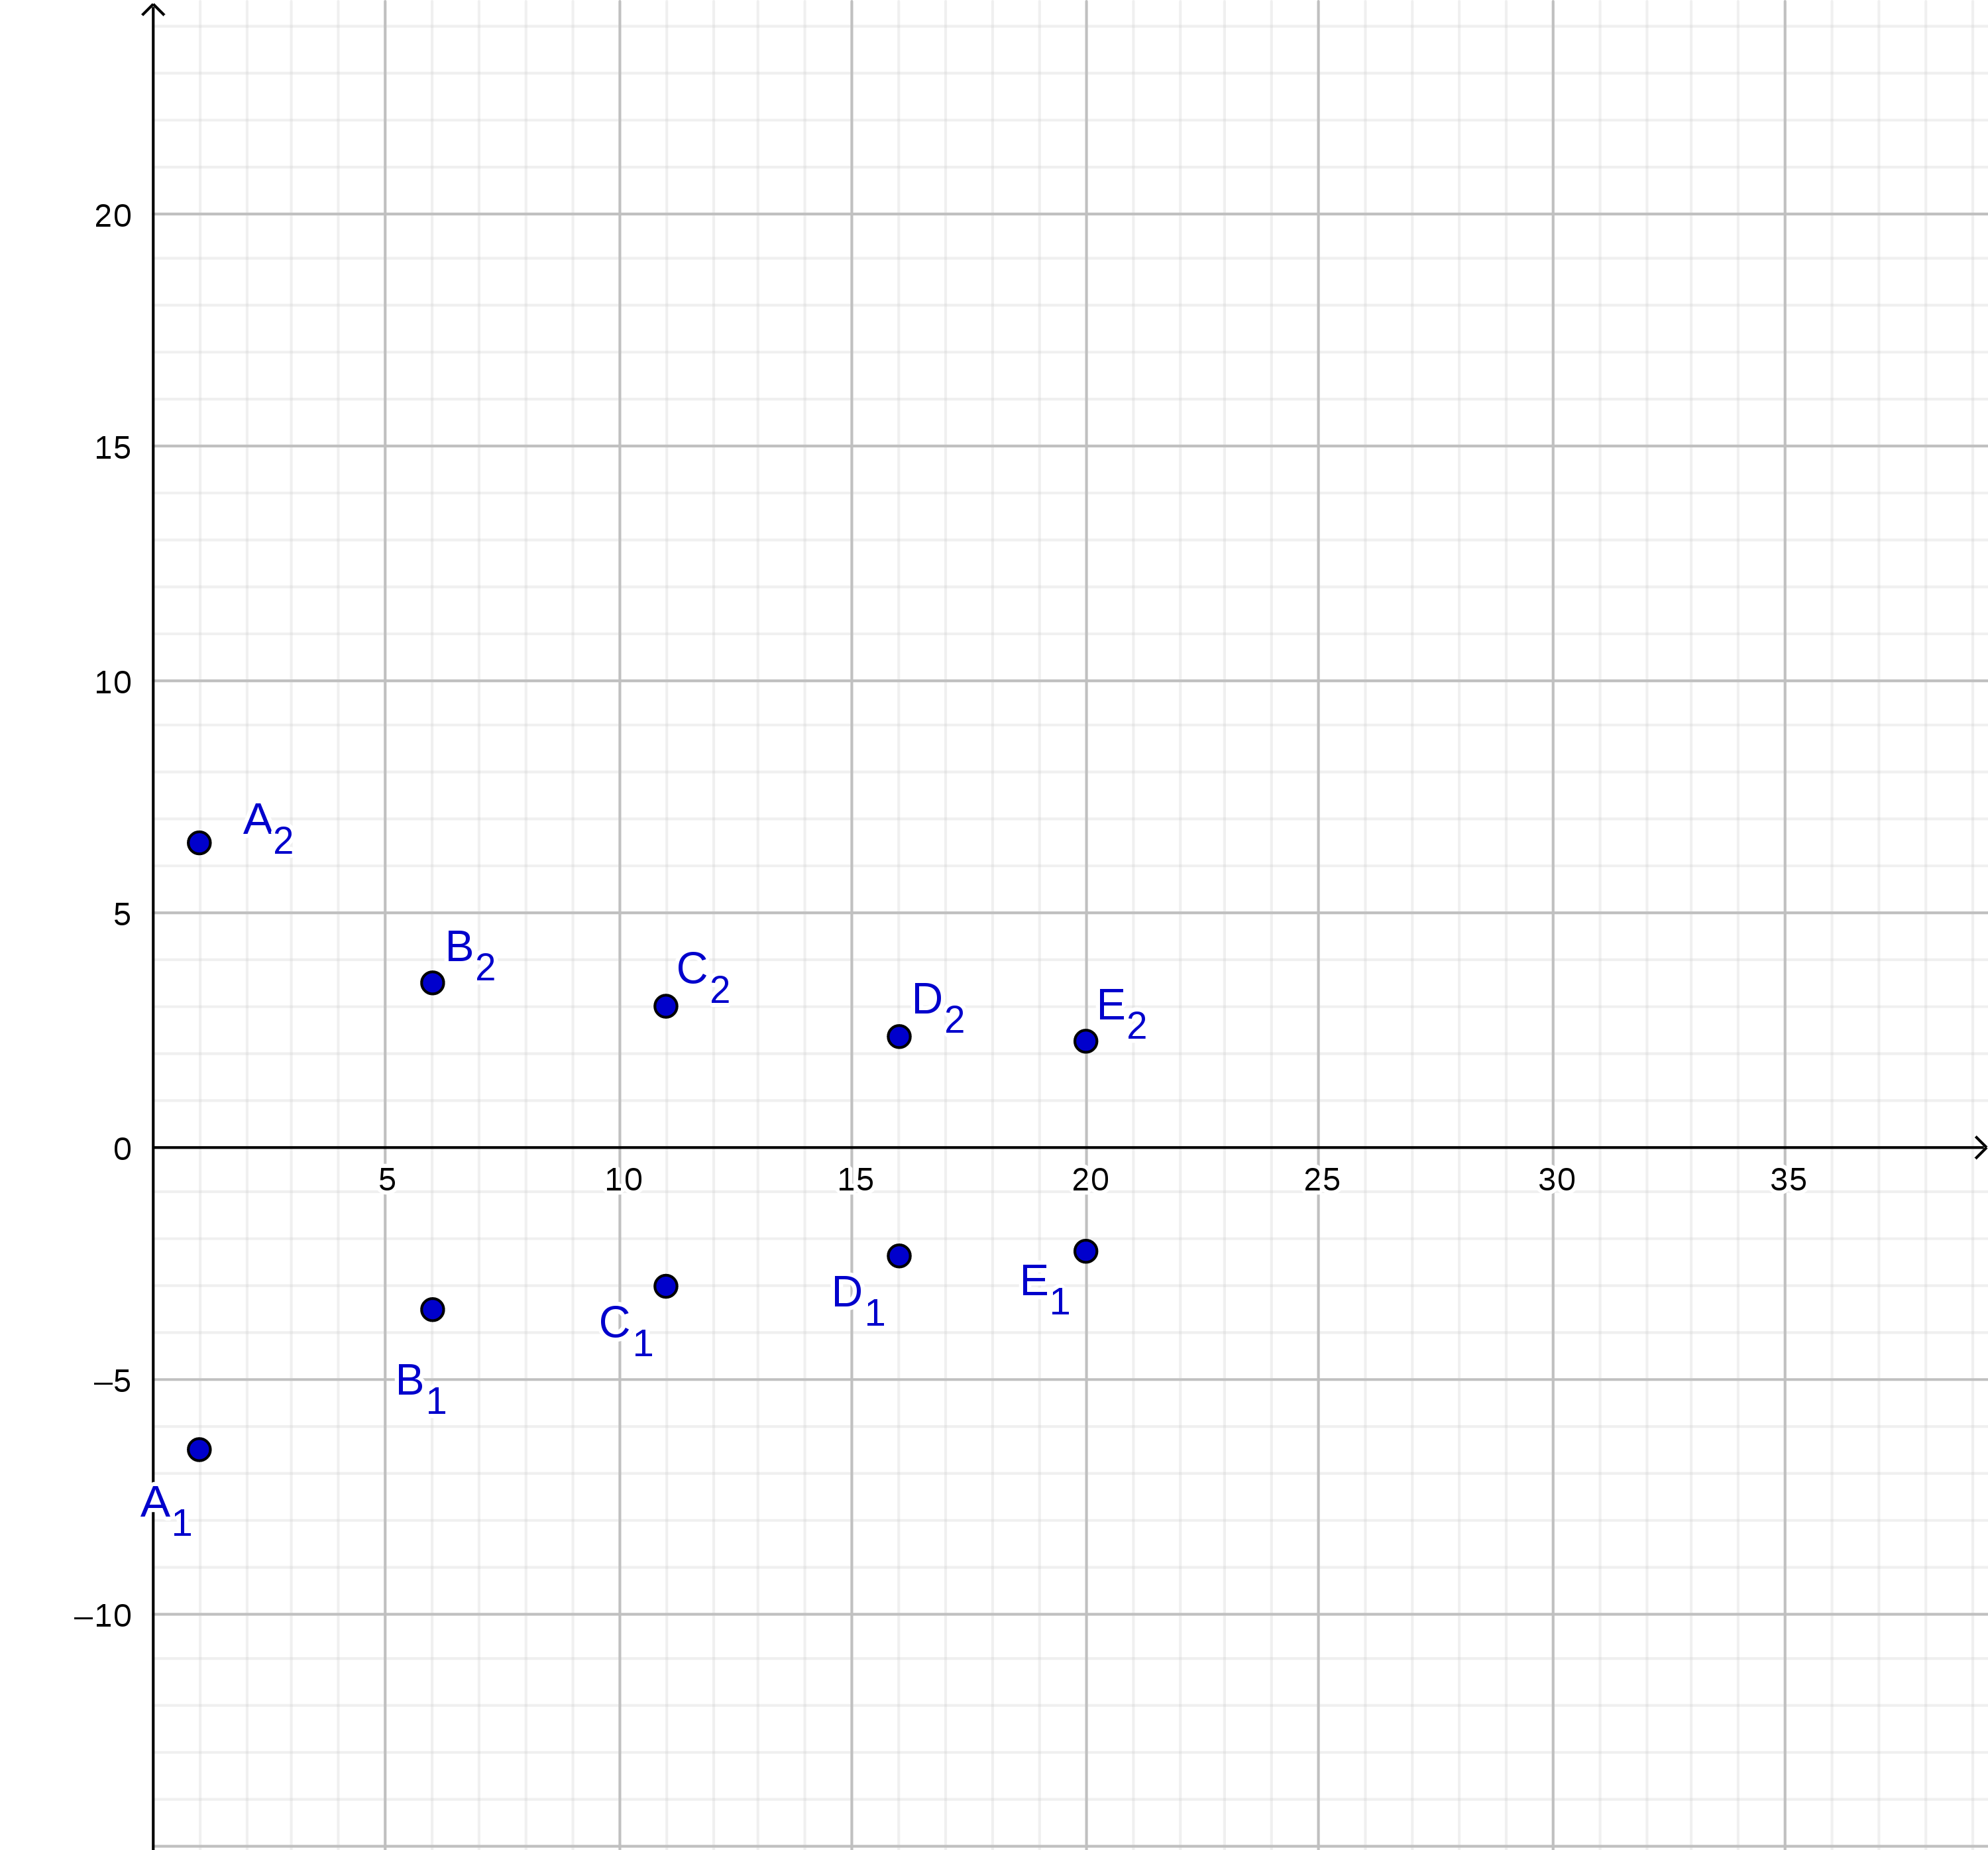
\includegraphics[width=90mm]{./images/2d-intersecao-circ-xy.png}
            %\caption{Interseção das circunferências com o plano $xy$}
            %\label{figu}
        %\end{figure}
%
        %Na tentativa de encontrar uma função derivável (porque a corneta "é derivável")
        %que atinja aproximadamente os pontos encontrados, sugerimos primeiramente:
        %$$ f(x) = \dfrac{1}{x}$$
        %E posteriormente:
        %$$ f(x) = \dfrac{a}{x^c} + b$$
        %Com $a,b,c \in \mathbb{R}$.
        %Utilizando os "sliders" do Geogebra, nos permite aproximar a corneta com 
        %$$ f(x) = \dfrac{6}{x^{0.4}} + 0.4$$
        %
        %\begin{figure}[ht!]
            %\centering
            %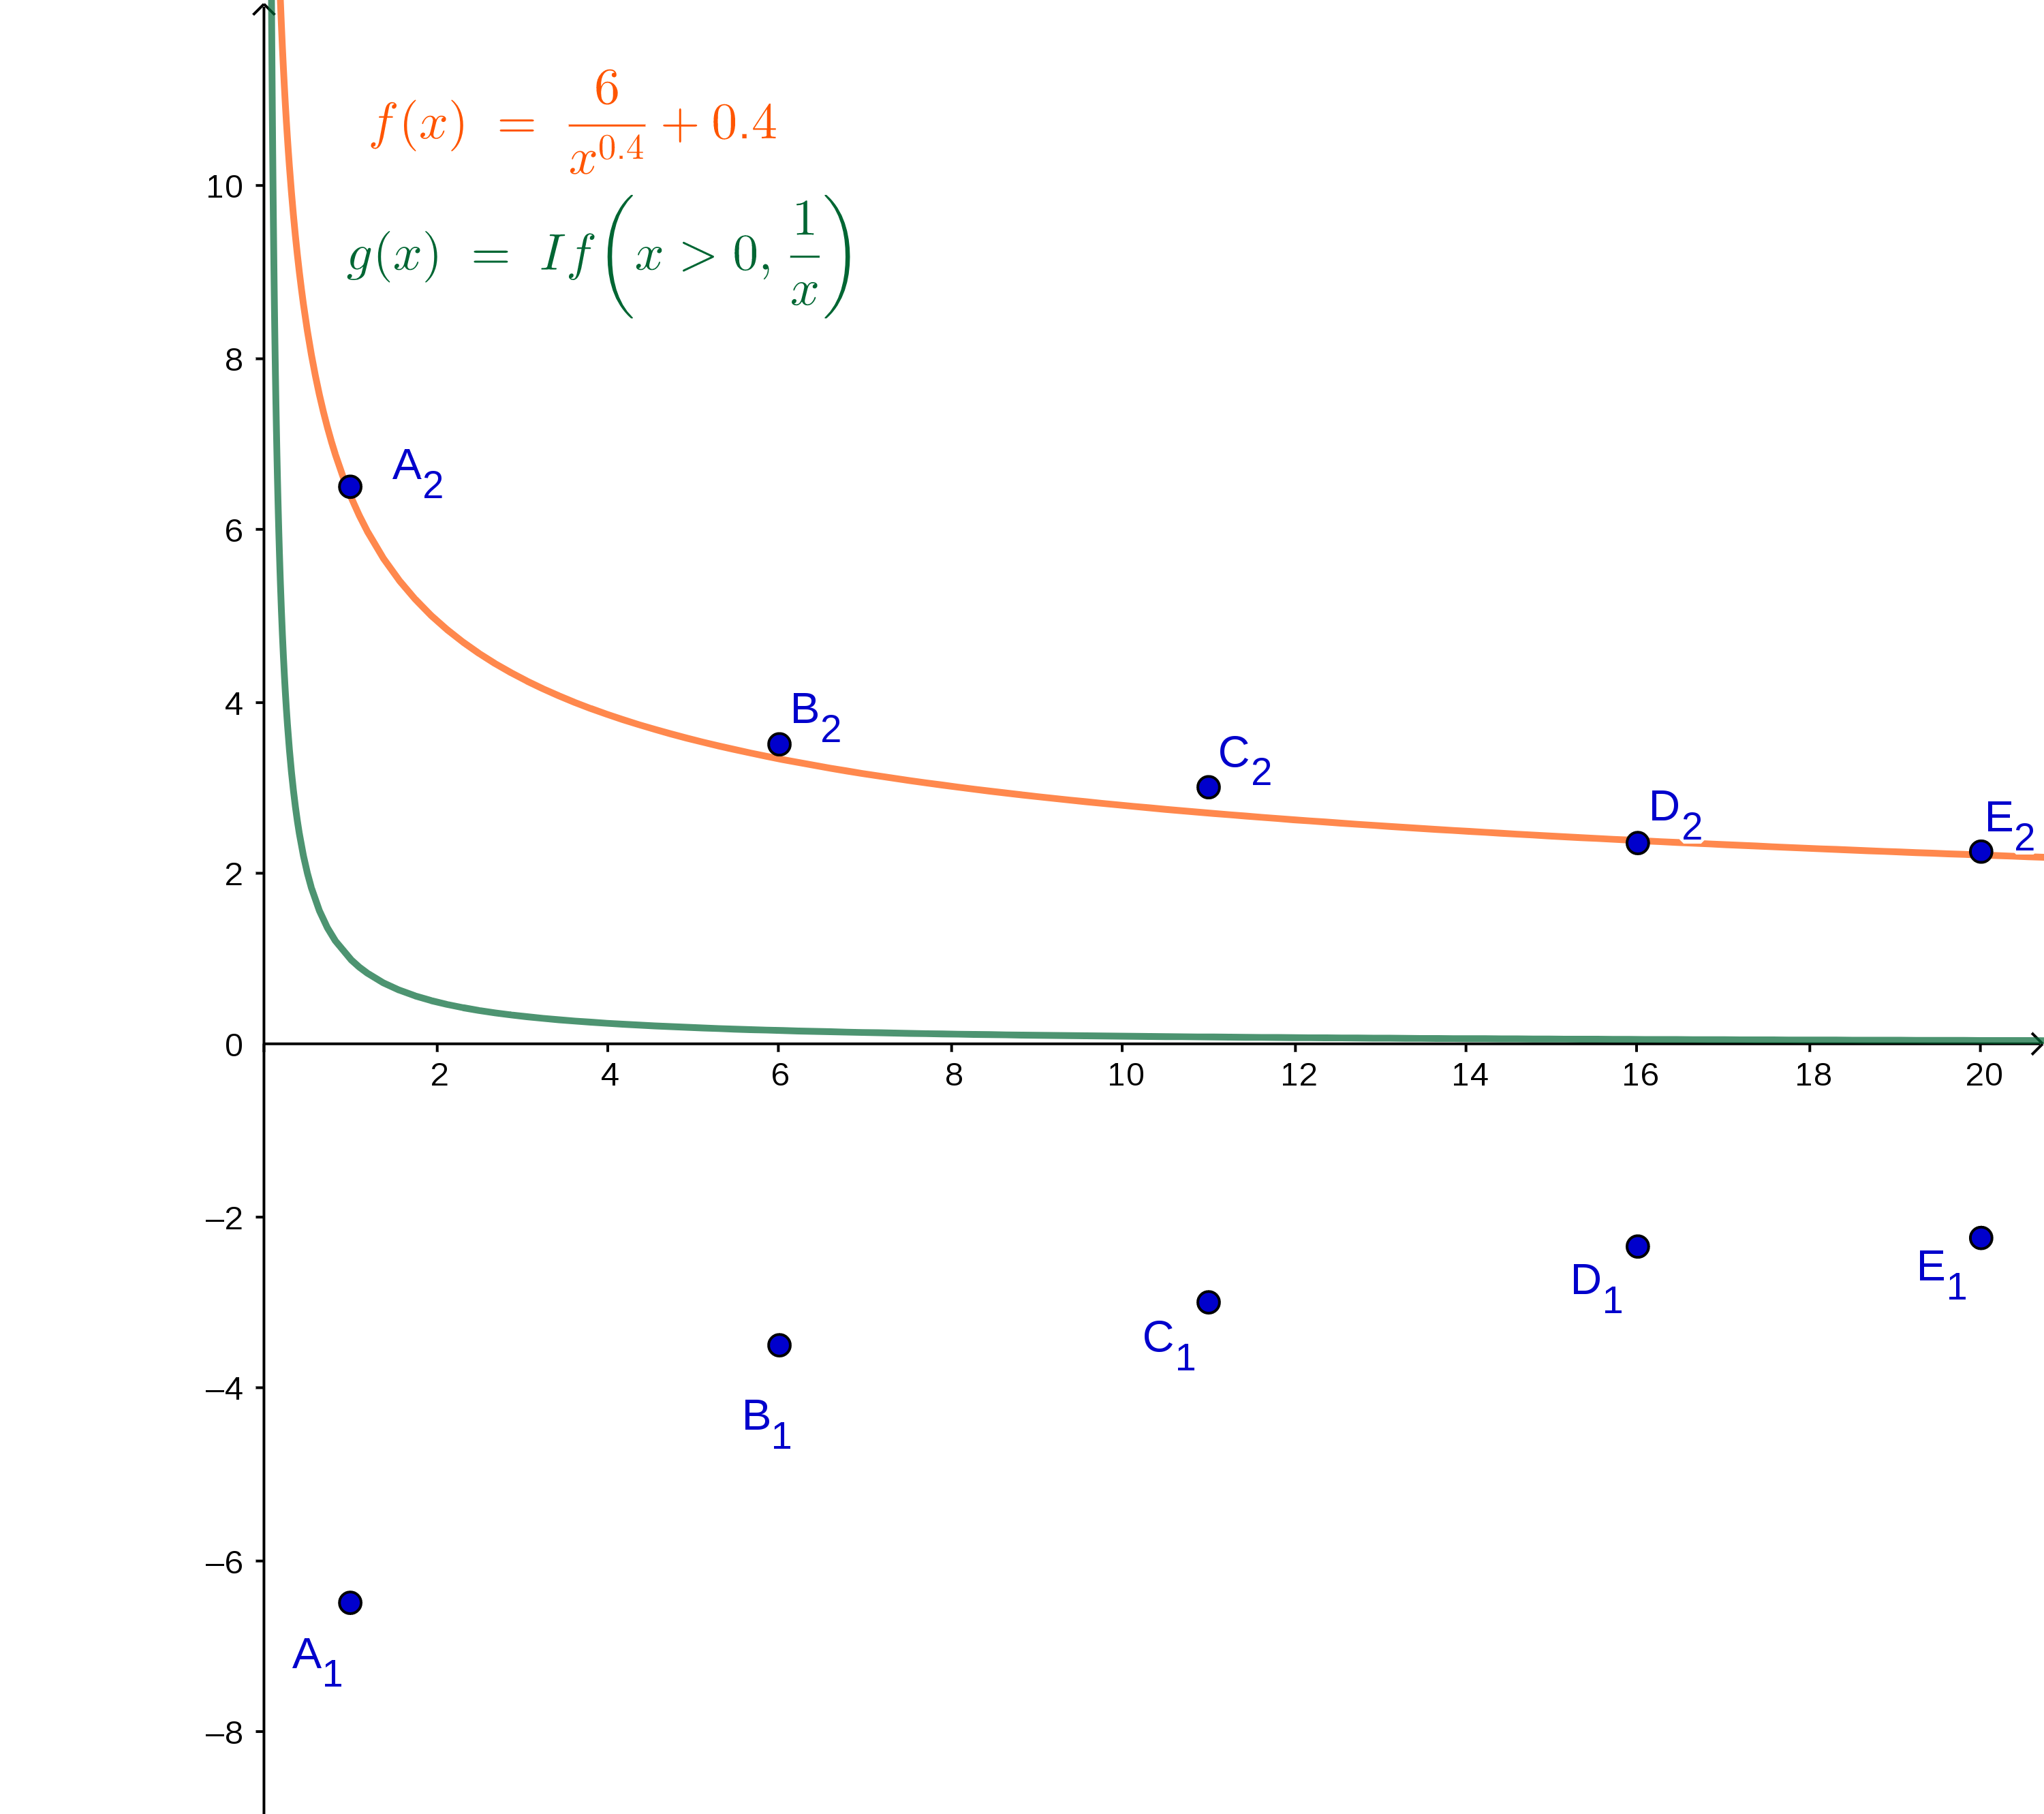
\includegraphics[width=90mm]{./images/2d-x-na-menos-um-e-aproximacao.png}
            %\caption{Aproximando os pontos com função \label{2d-x-na-menos-um-e-aproximacao}}
        %\end{figure}
        %
%
        %Por fim, basta limitar $f(x)$ no domínio e rotacionar usando o comando "surface", então obtemos:
        %
        %\begin{figure}[ht!]
            %\centering
            %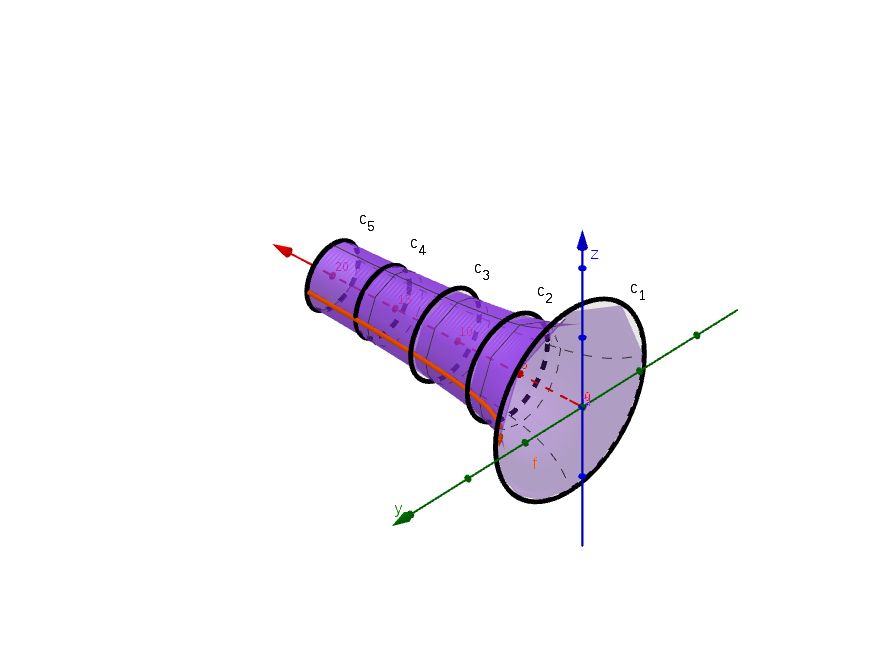
\includegraphics[width=90mm]{./images/3d-solido-pronto-e-funcao-geradora.png}
            %\caption{Sólido, função geradora, circunferências \label{3d-solido-funcao-circunferencias}}
        %\end{figure}
%
        %
        %Para obtermos o volume do sólido, temos:
        %$$ V = \pi \int_a^b[f(x)]^2 dx = \int_1^{20} \dfrac{6}{x^{0.4}} + 0.4 dx$$
        %$$ \int \dfrac{6}{x^{0,4}} + 0,4 dx = 0,4x + 10 x^{0,6} $$
        %$$ V = F(20) - F(1) = (0,4 \cdot 20 + 10 \cdot 20^{0,6}) - (0,4 + 10) \approx 57,94 u.v.$$
        %
    %%%%%%%%% Exercício 2 - Fim 
%
     %%%%%%%%% Exercicio 3 - Início
    %\item 
        %\begin{enumerate}
            %\item Se Leonard consegue  dar passos que atendem ao método de Zenão (ou Zeno), então talvez seja
                %possível que 
                %ele consiga também dar uma quantidade infinita de passos. Mas se ele não consegue 
                %dar infinitos passos, então ele não consegue atravessar o corredor utilizando o método de Zenão.
                %Mas suponhamos que os cinco primeiros passos ele utilize do método de Zenão, então no quinto passo
                %ele estará $\approx 1,2m$ distante, e quem dá um passo de $19m$ dá um passo de $2$ então ele atravessa.
            %\item
                %O corredor tem $d = 38.50m$ então, \\
                %Primeiro passo: $19.25m$ \\
                %Segundo passo: $28.875m$ 
            %\item 
                %\begin{align*}
                    %d_1 &= \dfrac{d}{2^1} = 19,25\\
                    %d_2 &= \dfrac{d}{2^1} + \dfrac{d}{2^2} \approx 28,87 \\
                    %d_3 &= \dfrac{d}{2^1} + \dfrac{d}{2^2} + \dfrac{d}{2^3} \approx 33,68 \\
                    %d_4 &= \dfrac{d}{2^1} + \dfrac{d}{2^2} + \dfrac{d}{2^3} + \dfrac{d}{2^4} \approx 36,09 \\
                    %d_5 &= \dfrac{d}{2^1} + \dfrac{d}{2^2} + \dfrac{d}{2^3} + \dfrac{d}{2^4} + \dfrac{d}{2^5} \approx 37,29 \\
                    %\\
                    %d_n &= \dfrac{d}{2^1} + \dfrac{d}{2^2} + \dfrac{d}{2^3} + \hdots + \dfrac{d}{2^n} \\
                        %&= d \cdot \sum_{i=1}^n 2^{-i} \\
                        %&= 38,50 \cdot \sum_{i=1}^n 2^{-i} 
                %\end{align*}
            %\item
                %Se as fórmulas que seguem representam o problema (com somas infinitas não se brinca, disseram), então sim.
                %$$ 38,50 - 38,50 \sum_{i=1}^n 2^{-i} < 38,50 \epsilon \iff 1 - \sum_{i=1}^n 2^{-i} < \epsilon $$
                %Dado um $\epsilon$ qualquer, vamos escolher um novo e chamá-lo pelo mesmo símbolo, 
                %tal que é o maior $2^{-k}$ que seja menor que o $\epsilon$ anterior, com $k$ natural.
                %Vamos provar para todo $\epsilon$ dado existe $n$ tal que vale:
                %$$1 < \sum_{i=1}^n 2^{-i} + \epsilon $$
                %\begin{proof}
                %Tomando $n = k+1$, por indução sobre $k$ se $k = 1$:
                %$$\sum_{i=1}^{k+1} 2^{-i} + \dfrac{1}{2^k} =
                    %\sum_{i=1}^{1+1} 2^{-i} + \dfrac{1}{2^1} =
                    %\dfrac{1}{2^1} + \dfrac{1}{2^2} + \dfrac{1}{2^1} > 1 $$
                %Nossa hipótese de indução é que existe um $k_0 = k$ tal que:
                %$$ \sum_{i=1}^{k+1} 2^{-i} + \dfrac{1}{2^k} > 1$$ 
                %Provemos que vale também para $k+1$
                %\begin{align*}
                    %& \sum_{i=1}^{(k+1)+1} 2^{-i} + \dfrac{1}{2^{(k+1)}} = \\
                    %%& \sum_{i=1}^{k} 2^{-i} + \dfrac{1}{2^{k+1}} + \dfrac{1}{2^{k+2}} + \dfrac{1}{2^{(k+1)}} = \\
                    %& \sum_{i=1}^{k} 2^{-i}\dfrac{1}{2^{k+1}} + \dfrac{1}{2^{k+2}} + \dfrac{1}{2^{(k+1)}} = \\
                    %& \left( \sum_{i=1}^{k} 2^{-i} \dfrac{2 \cdot 1}{2^{k+1}} \right) + \dfrac{1}{2^{k+2}}  > 1
                %\end{align*}
                %\end{proof}
            %\item
                %Se ele fosse dando um passo após o outro, ele chega cada vez mais próximo, até o momento em que ele para de 
                %andar com o método de Zenão e dá um passo que chega no final do corredor ou o atravessa.
            %\item
                %$$ 38,50 - 38,50 \sum_{i=1}^n 2^{-i} $$
                %Desconsiderando a subtração, a primeira parcela da soma é a distância a percorrer e a 
                %segunda é o passo $n$ que pode ser entendida como
                %uma função na variável $d$.
                %No exercício (d) mostramos que Leonard pode aproximar-se arbitrariamente do final do corredor tanto quanto
                %se queira. Isso pode ser representado dizendo que o limite das somas parciais da série cujos termos são 
                %os tamanhos dos passos é convergente, e "converge para o fim do corredor".
                %Note que também pode ser argumentado que a série é um múltiplo da série geométrica com base menor que 1.
        %\end{enumerate}
        %%%%%%%%%%%% Exercicio 3 - Fim  
%\end{enumerate}
%%\begin{enumerate}
%%    %\item
%%        %Primeiro consideraremos algumas fórmulas antes de começar a dedução.
%%        %$ d(P_i, P_{i-1}) = \sqrt{ 1+ f'(x_i^*} \cdot \Delta x $ onde $x^*$ é algum ponto do domínio de $f$ \\
%%        %$ A_l = 2\pi g$
%%        %onde $r$ é $ (raio maior + raio menor)/2$ e $g$ é a geratriz do tronco de cone.
%%%
%%        %Deduziremos a fórmula de uma função $f$ que é contínua.
%%%
%%        %A ideia é considerar o limite quando $\Delta x \rightarrow 0$ e calcular a área do tronco de cone.
%%%
%%        %Consideraremos $P_j$ pontos da curva que será feita revolução.
%%%
%%        %$$f(x_i) \approx f(x_i^*) \approx f(x_{i-1}) $$
%%        %$$A_i = 2\pi \left( \dfrac{ f(x_i) + f(x_{i-1} }{2} \right) \cdot d(P_i, P_{i-1}) \approx $$
%%
%%
%%    \item
%%    Considerando a função
%%    $$ f(x,y) = \dfrac{(x-1)^2 + x(y+1)^2} {(x-1)^2+(y+1)^2}$$
%%    primeiramente vamos pegar um $\epsilon$ “qualquer” (considerando as capacidades 
%%    do Geogebra) usando o “slider”, que nesta atividade está variando de $0.1$
%%    até $0.5$. 
%%    
%%    Sabendo que o limite da função quando $f \rightarrow (1,-1)$ é igual a 1, temos pela definição de limite:
%%    $\abs{ f(x,y) - 1 } < \epsilon  \iff -\epsilon + 1 < f(x,y) < \epsilon + 1$
%%    Se considerarmos $-\epsilon+1$ e $\epsilon + 1$ como a terceira coordenada de um
%%    plano cada um, temos que $\epsilon + 1$ é o plano verde, e $- \epsilon + 1$
%%    é o plano amarelado na figura abaixo.
%%
%%    \begin{figure}[ht!]
%%        \centering
%%        \includegraphics[width=90mm]{img1.png}
%%        \caption{Intersecção e projeção no plano $xy$ \label{intersecao}}
%%    \end{figure}
%%
%%    Ainda considerando a Figura \ref{intersecao}, temos em roxo o gráfico de $f$, também as
%%    intersecções de $f$ com os planos, e a translação da intersecção de $f$ com os planos, no plano $xy$.
%%    A reta preta que passa por $A$ é uma reta perpendicular a $xy$.
%%    
%%    \newpage
%%    \begin{figure}[ht!]
%%        \centering
%%        \includegraphics[width=90mm]{img2.png}
%%        \caption{Projeção da intersecção \label{projecao}}
%%    \end{figure}
%%    Na figura \ref{projecao}, temos a translação das interseções dos planos com $f$ no plano
%%    $xy$, que estão de cores verde e amarelo. Tem-se então que há duas distâncias, do 
%%    ponto $A$ até a translação amarela, e outra de $A$ até a translação verde. 
%%    Pegando a menor delas, conseguimos fazer como na Figura
%%    \ref{imagem_entre_planos}, a seguir, onde todo
%%    o gráfico de $f$, restrito ao círculo (aberto) preto, está entre os planos verde e amarelo.
%%    \begin{figure}[ht!]
%%        \centering
%%        \includegraphics[width=90mm]{img3.png}
%%        \caption{Imagem de $f$ entre os planos $\epsilon+1$ e $-\epsilon + 1$
%%        \label{imagem_entre_planos}}
%%    \end{figure}
%%    \item
%%        Consideraremos a função 
%%        $$ f(x,y) = x^2y^2 , x\neq 0 \neq y$$
%%        Sejam 
%%        $$\pi_1: y=1$$ 
%%        $$ C_1 = \pi_1 \cap f $$
%%        Temos 
%%        \begin{equation}
%%           C_1: y=1 \land x^2y^2=z \iff C_1: x^2=z, y=1
%%        \end{equation}
%%        $C_1$ é a interseção de $f$ com $\pi_1$ e sua derivada parcial, que nos
%%        dá o valor do ângulo da reta tangente em cada um de seus pontos é dada
%%        por:
%%        $$ \dfrac{\partial y^2x^2}{\partial x} = y^22x \leadsto 1\cdot2\cdot
%%        (-1) = -2$$
%%        Portanto $-2$ é o valor do ângulo da reta tangente à $C_1$ considerando
%%        o eixo de referência $z=0, y=1, x=x$.
%%
%%        De (1) temos a equação de $C_1$ e sua derivada parcial no ponto $(-1,1)$. Agora queremos
%%        descobrir a reta $r_1$ tangente à $C_1$.
%%        
%%        Pelo desenvolvimento, ocorre $r_1 \subset \pi_1$, pois $$( \pi_1 \cap f)
%%        \subset\pi_1 $$ e portantanto, a derivada de uma curva do plano, se existir, estará contida no plano.
%%
%%        Conseguimos determinar que $r_1 \subset \pi_1$, agora prossigamos com a
%%        fórmula da reta no plano:
%%        $$ z - z_0 = \alpha ( x - x_0) \iff
%%        z - f(x_0,y_0) = \dfrac{\partial f(-1,1)}{\partial x} \cdot (x-x_0) $$
%%        que substituindo os valores temos:
%%        $$ z - 1 = -2\left(x-(-1)\right) \iff z = -2x-1 $$
%%        Então temos que $r_1: y=1 \land z=-2x-1$
%%
%%        Analogamente encontramos $C_2$ e $r_2$, que são:
%%        $$ C_2: z=y^2$$
%%        $$r_2: x=-1 \land z=y^2$$
%%
%%        Sabendo que duas retas concorrentes determinam um único plano, e sabendo
%%        que o vetor normal de um plano é dado pelo produto vetorial de quaisquer
%%        dois vetores não múltiplos entre si, temos:
%%
%%        $$\overrightarrow{\rm n_{\pi}} = \overrightarrow{\rm v_1} \times
%%        \overrightarrow{\rm v_2}$$
%%        onde $\overrightarrow{\rm v_1}$ e $\overrightarrow{\rm v_2}$ são vetores
%%        diretores de $r_1$ e $r_2$, e $\pi$ é o plano tangente no ponto
%%        considerado. E ainda, desconsideramos que o vetor normal não é
%%        único, mas este é um vetor normal e é suficiente.
%%
%%        Por brevidade, usaremos a fórmula para obter o vetor normal:
%%        $$\overrightarrow{\rm n_{\pi}} = \left(- \dfrac{\partial f(-1,1)}{\partial x} ,
%%        - \dfrac{\partial f(-1,1)}{\partial y},
%%        1 \right)$$
%%
%%        Da equação geral do plano: $ax + by + cz + d = 0$, substituindo os
%%        valores temos:
%%        $$ 2(-1) -2(1) + 1(1) + d = 0 \implies d = 3$$
%%        E a equação do plano tangente é:
%%        $$ +2x - 2y +z + 3 = 0 $$
%%        
%%        A Figura \ref{plano_tangente} ilustra a função e o plano tangente:
%%
%%    \begin{figure}[ht!]
%%        \centering
%%        \includegraphics[width=90mm]{img4.png}
%%        \caption{Plano tangente \label{plano_tangente}}
%%    \end{figure}
\end{enumerate}
\end{document}

